% !TEX encoding = UTF-8 Unicode 
% !TEX root = praca.tex

\chapter{Research discussion}

In this chapter, the results from the performed experiments are aggregated, presented in a visual form, and analyzed in accordance with the purpose and scope of this thesis. The analysis outcome became a base for forming final conclusions.

\section{Experiment results analysis}

In the following sections, firstly the average metric values are calculated to perform the overall comparison between the technologies. Afterward, each research scenario is considered separately.

% !TEX encoding = UTF-8 Unicode 
% !TEX root = praca.tex

\subsection{Generalized results analysis}

CPU usage is a significantly valuable metric, especially for low-end devices, because it directly affects power consumption, and batteries in low-end devices are usually of smaller capacity.

\begin{figure}[H]
    \begin{minipage}{.48\textwidth}
        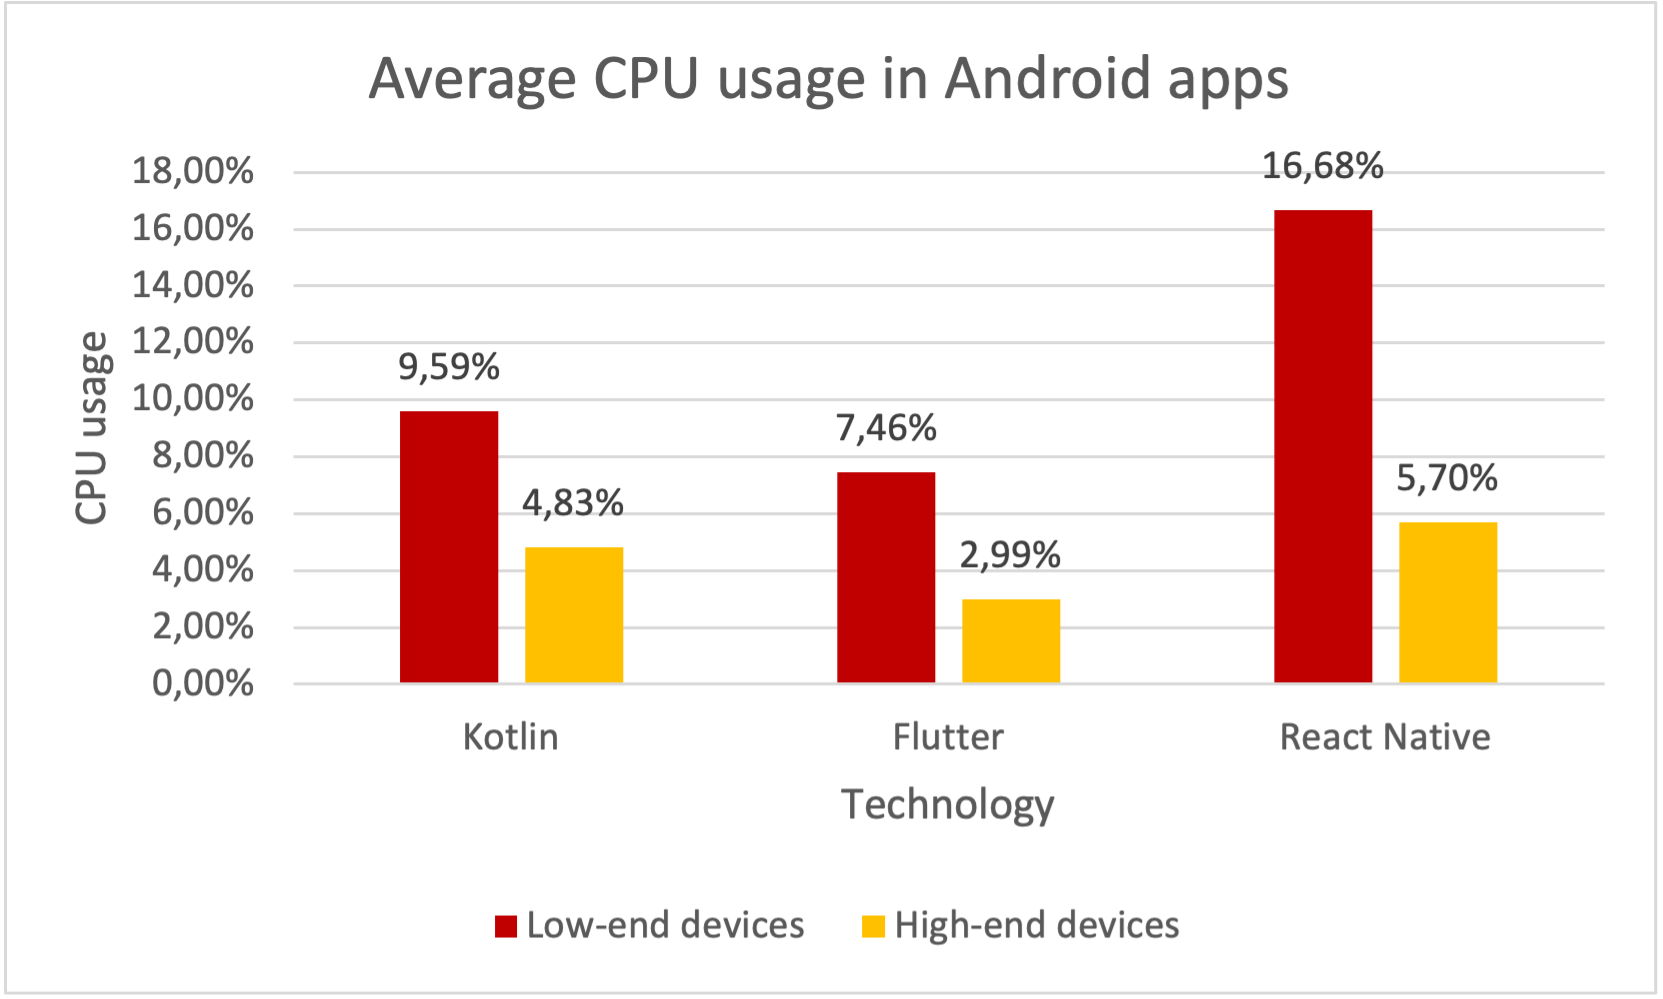
\includegraphics[width=\textwidth]{img/cpu_average_android}
        \caption{Average CPU usage in Android apps (Source: Own work)}
        \label{fig:cpu_avg_android}
    \end{minipage}
    \hfill
    \begin{minipage}{.48\textwidth}
        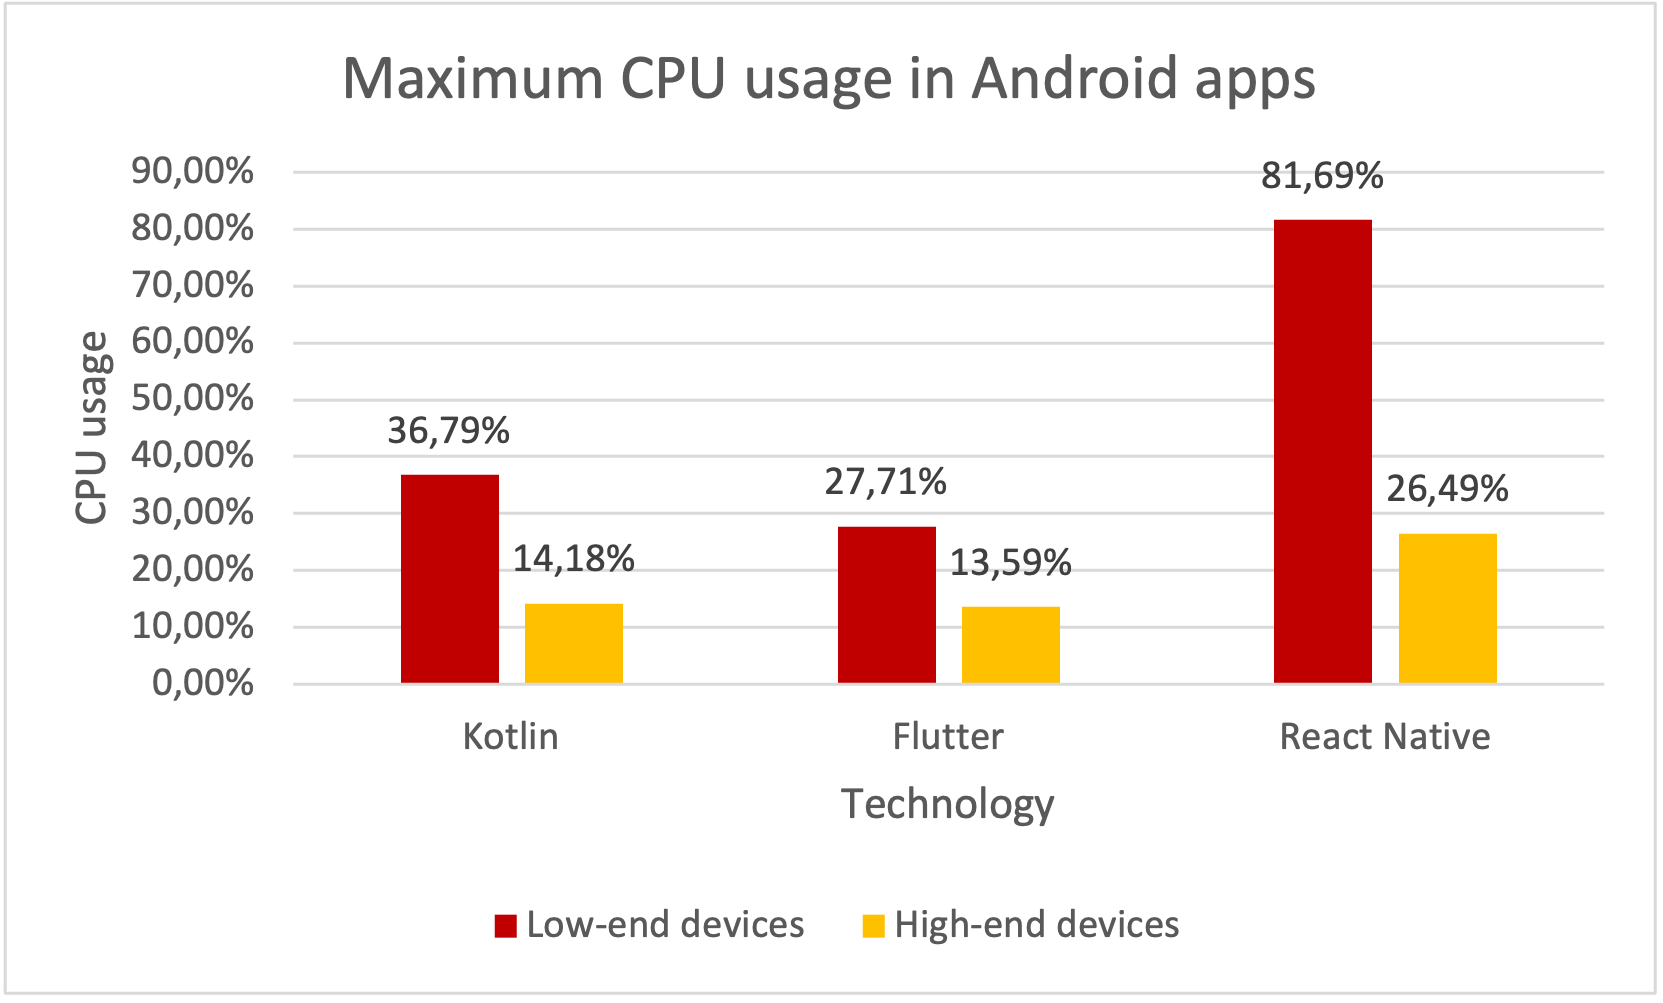
\includegraphics[width=\textwidth]{img/cpu_max_android}
        \caption{Maximum CPU usage in Android apps (Source: Own work)}
        \label{fig:cpu_max_android}
    \end{minipage}
\end{figure}

Figures \ref{fig:cpu_avg_android} and \ref{fig:cpu_max_android} show the comparison of CPU usage among Android apps developed with Kotlin, Flutter, and React Native. Overall, Flutter apps require the least CPU capacity across both low-end and high-end devices, thus implying the most efficient utilization of system resources. Kotlin apps perform slightly worse than Flutter apps, but they still do not exceed even 10\% of CPU usage, which is a great result. React Native apps show the highest CPU usage, most notably on low-end devices. Furthermore, they experience the highest spikes, reaching over 80\%. Such spikes may be concerning if they keep happening regularly. Kotlin and Flutter apps exhibit much lower maximum CPU usage.

\begin{figure}[H]
    \begin{minipage}{.48\textwidth}
        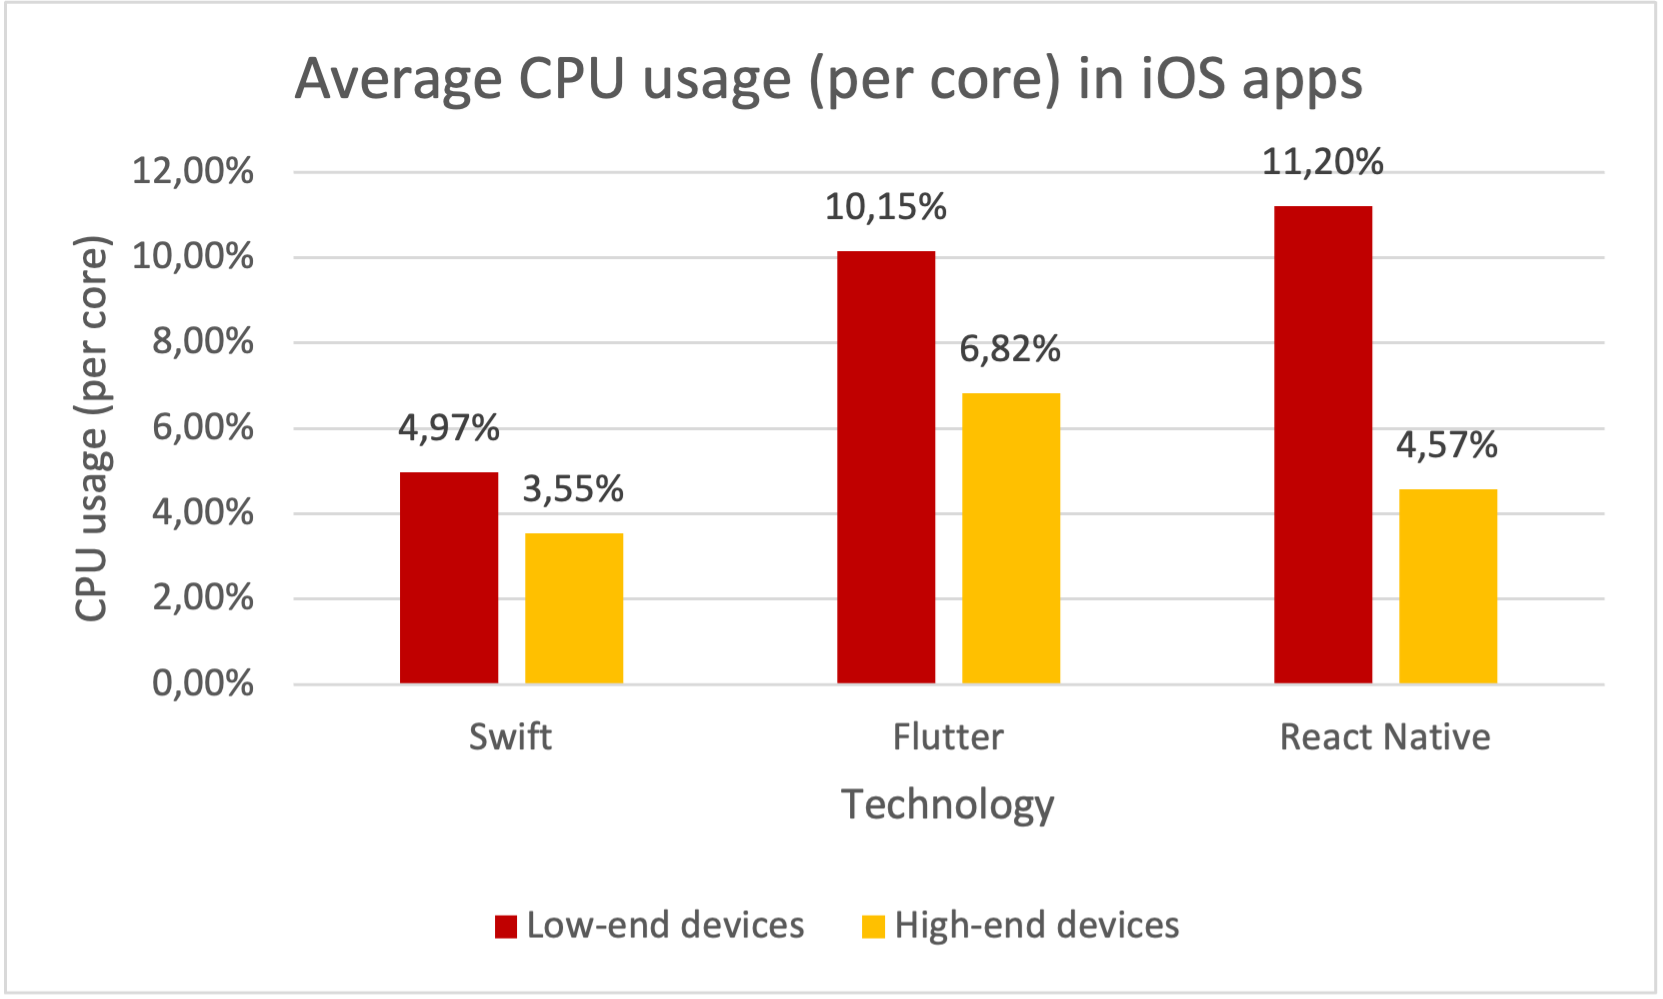
\includegraphics[width=\textwidth]{img/cpu_average_ios}
        \caption{Average CPU usage in iOS apps (Source: Own work)}
        \label{fig:cpu_avg_ios}
    \end{minipage}
    \hfill
    \begin{minipage}{.48\textwidth}
        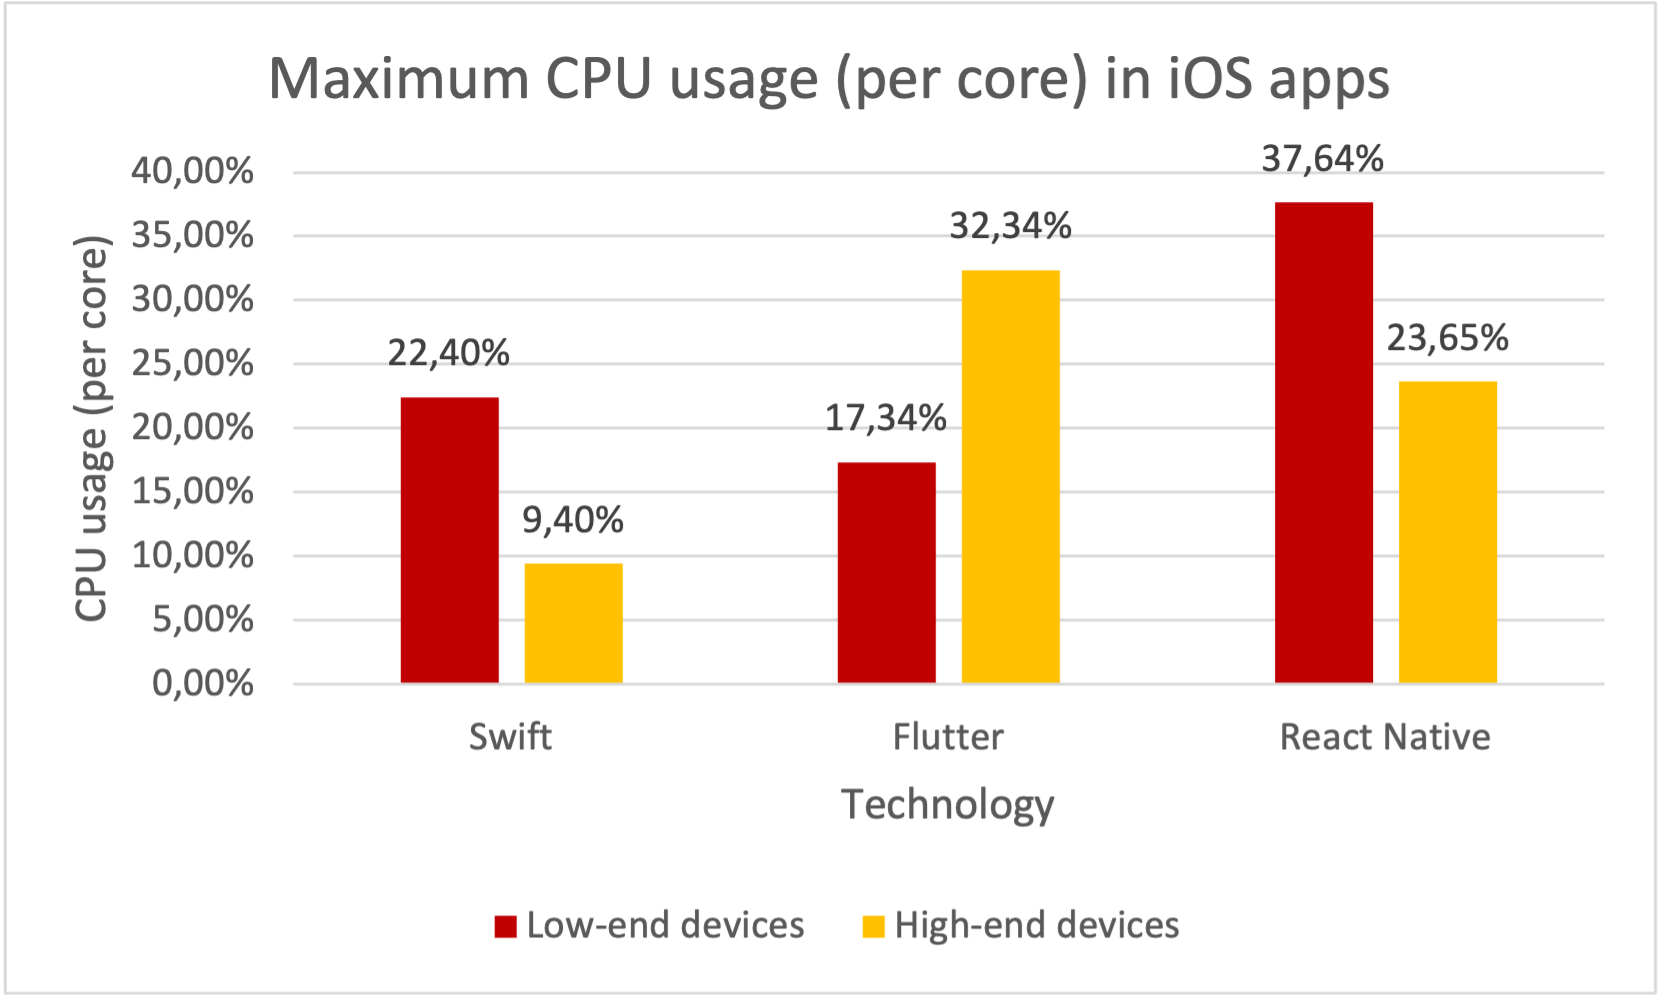
\includegraphics[width=\textwidth]{img/cpu_max_ios}
        \caption{Maximum CPU usage in iOS apps (Source: Own work)}
        \label{fig:cpu_max_ios}
    \end{minipage}
\end{figure}

Figures \ref{fig:cpu_avg_ios} and \ref{fig:cpu_max_ios} show the comparison of CPU usage among iOS apps developed with Swift, Flutter, and React Native. Swift apps perform the best on both low-end and high-end devices, with the average CPU usage remaining just under 5\% per core. Flutter apps and React Native apps exhibit similar results, although the former perform better on low-end devices and the latter perform better on high-end devices. However, React Native apps demonstrate the highest CPU usage spikes, similar to their Android equivalents.

\begin{figure}[H]
    \begin{minipage}{.48\textwidth}
        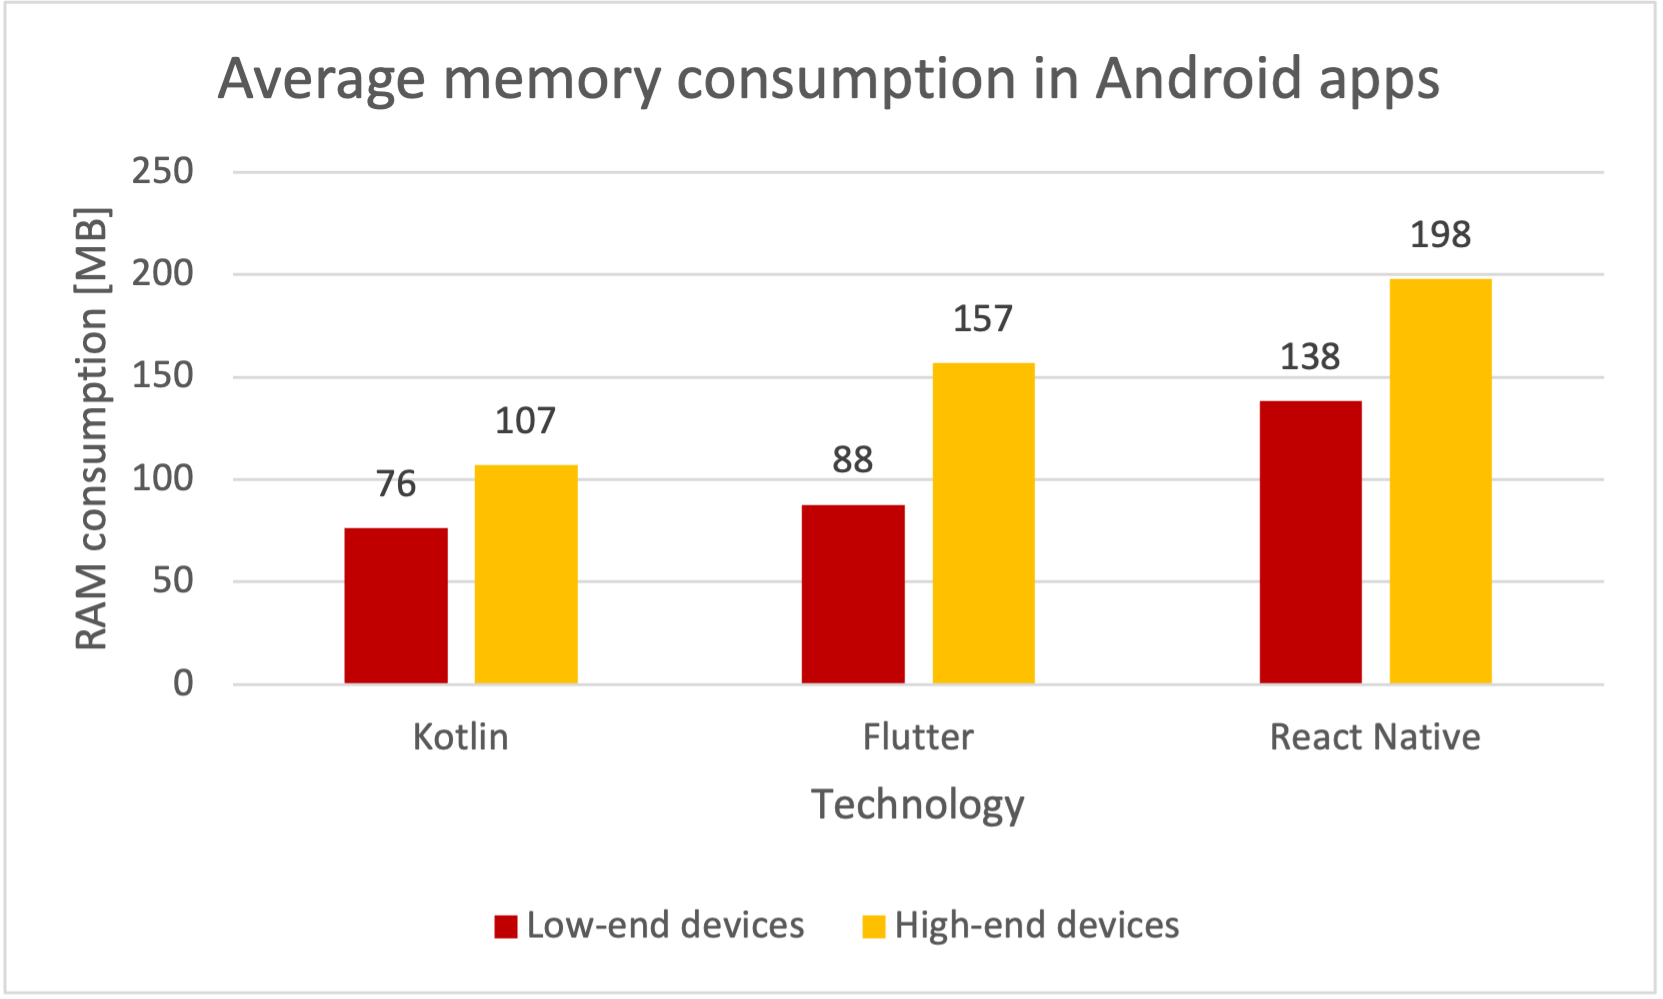
\includegraphics[width=\textwidth]{img/ram_average_android}
        \caption{Average memory consumption in Android apps (Source: Own work)}
        \label{fig:ram_avg_android}
    \end{minipage}
    \hfill
    \begin{minipage}{.48\textwidth}
        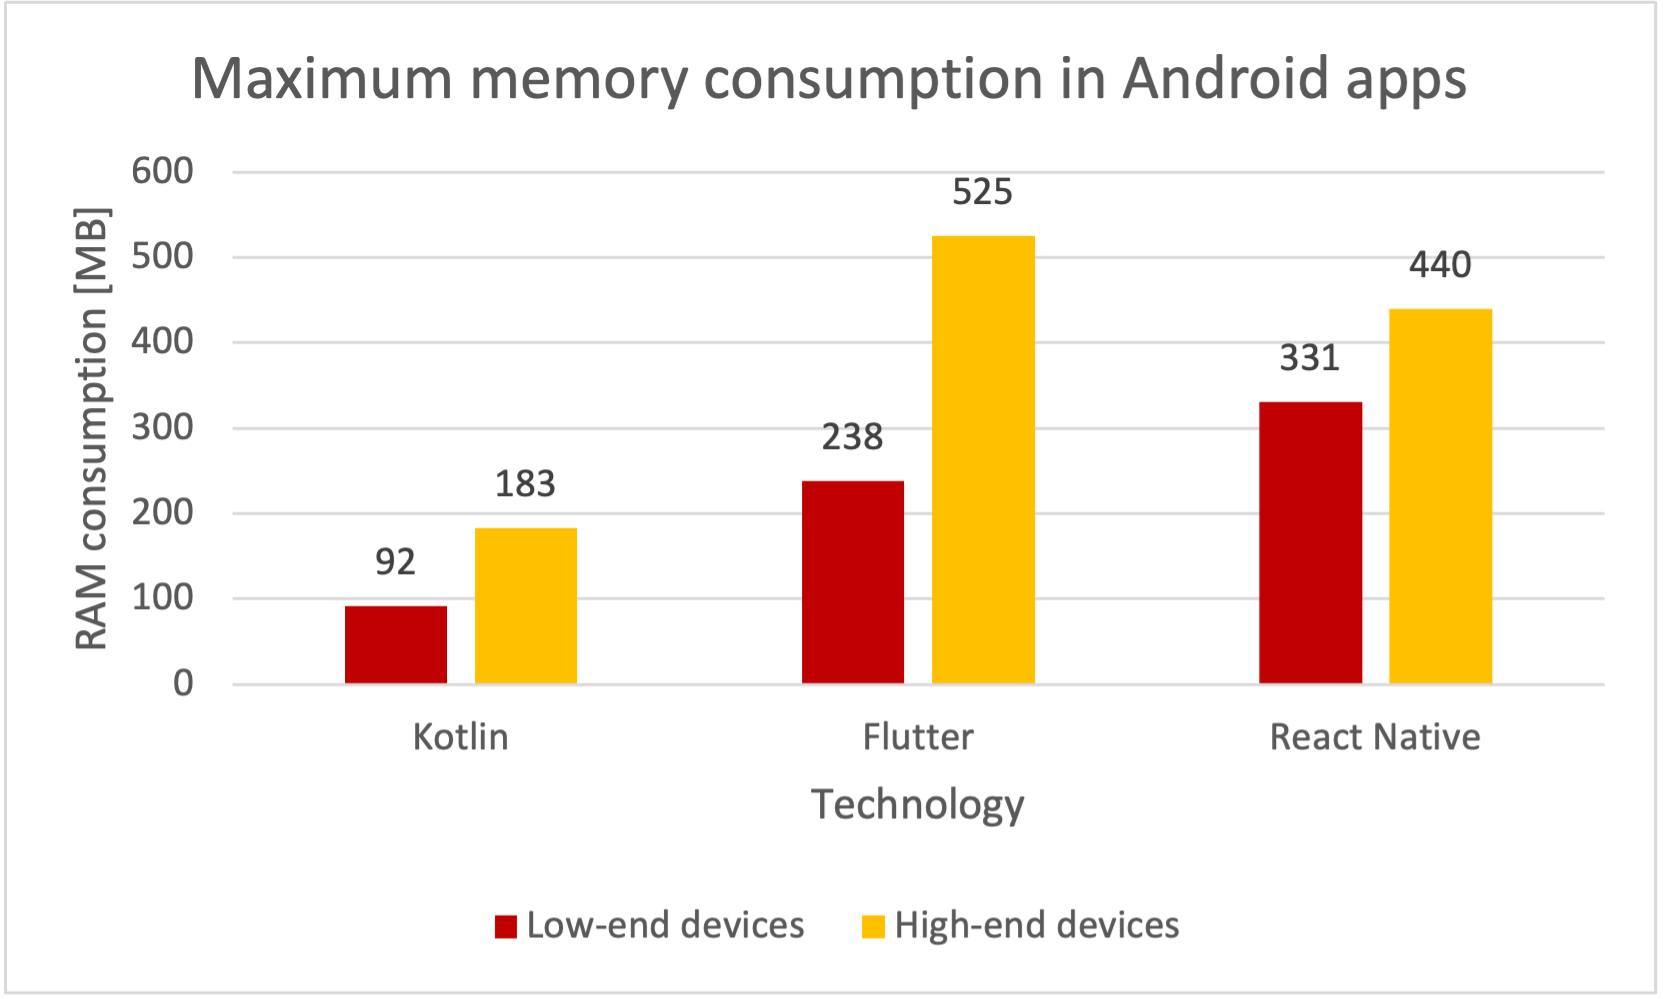
\includegraphics[width=\textwidth]{img/ram_max_android}
        \caption{Maximum memory consumption in Android apps (Source: Own work)}
        \label{fig:ram_max_android}
    \end{minipage}
\end{figure}

Figures \ref{fig:ram_avg_android} and \ref{fig:ram_max_android} show the comparison of memory consumption among Android apps developed with Kotlin, Flutter, and React Native. It can be observed that each technology has a similar ratio of memory used by low-end devices to memory used by high-end devices. Overall, Kotlin apps utilize the least memory resources, followed by Flutter apps, and then React Native apps. However, Flutter apps experience the highest spikes in RAM consumption, with the maximum reaching 525 MB on high-end devices as compared to Kotlin apps 183 MB. Nevertheless, high-end devices currently offer a solid amount of memory; therefore, such values (if sporadic) do not have to mean performance issues. Maximum memory usage should be tracked primarily on low-end devices.

\begin{figure}[H]
    \begin{minipage}{.48\textwidth}
        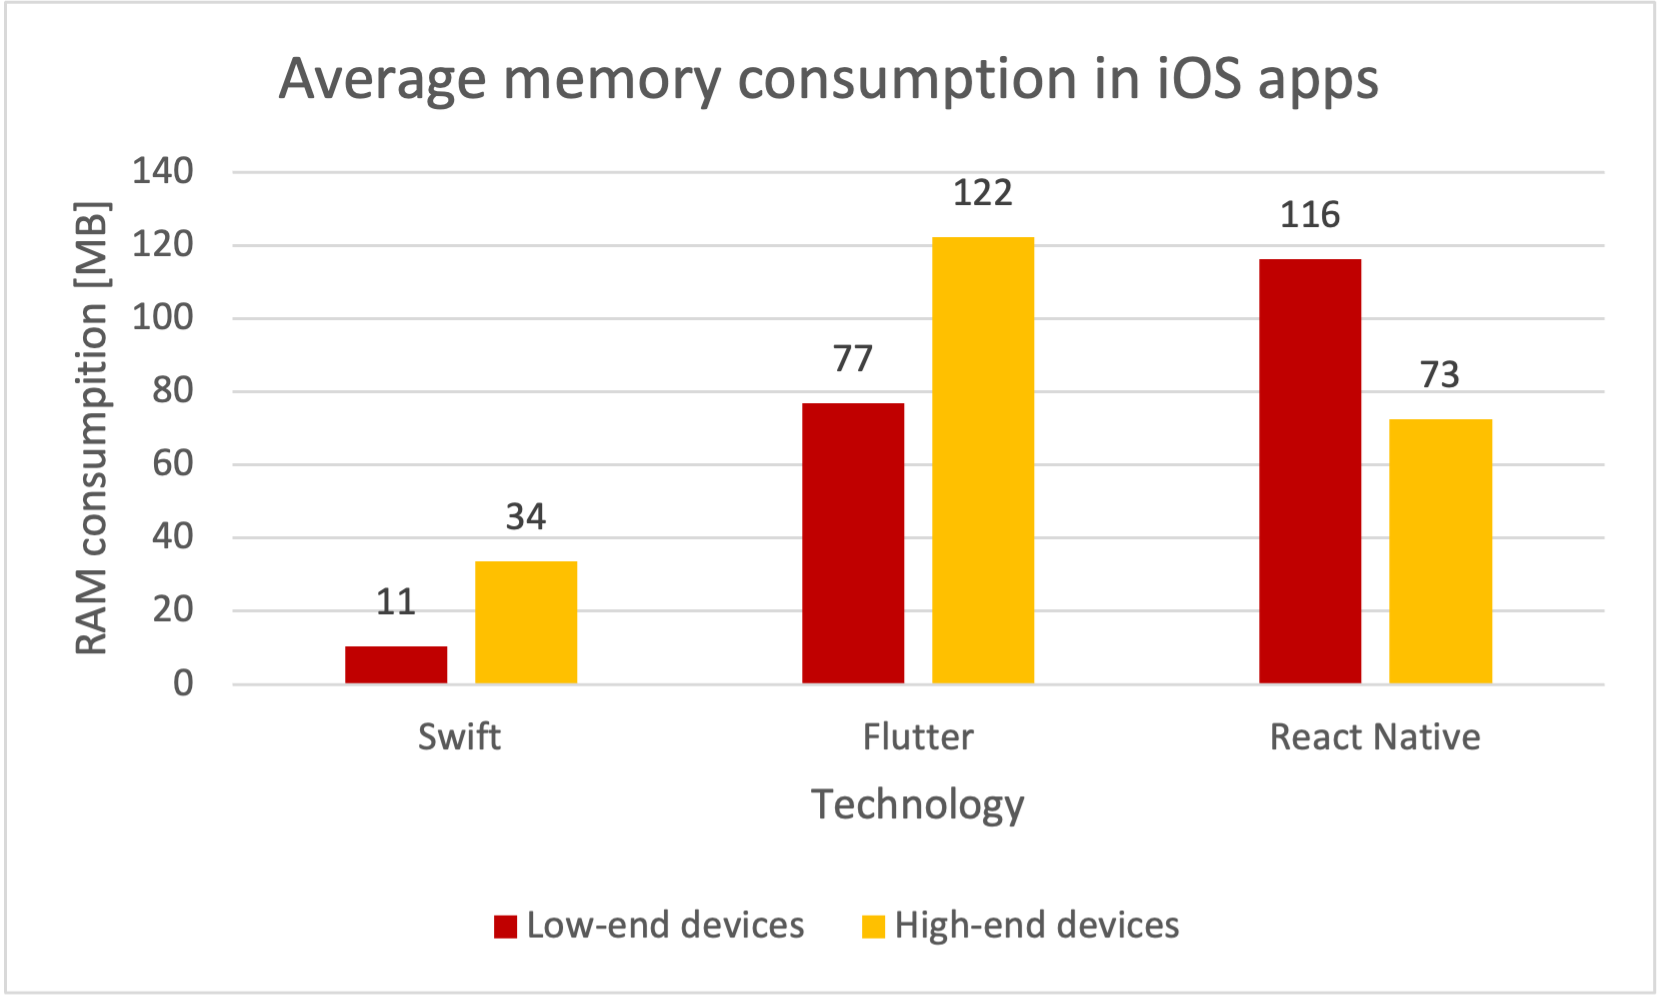
\includegraphics[width=\textwidth]{img/ram_average_ios}
        \caption{Average memory consumption in iOS apps (Source: Own work)}
        \label{fig:ram_avg_ios}
    \end{minipage}
    \hfill
    \begin{minipage}{.48\textwidth}
        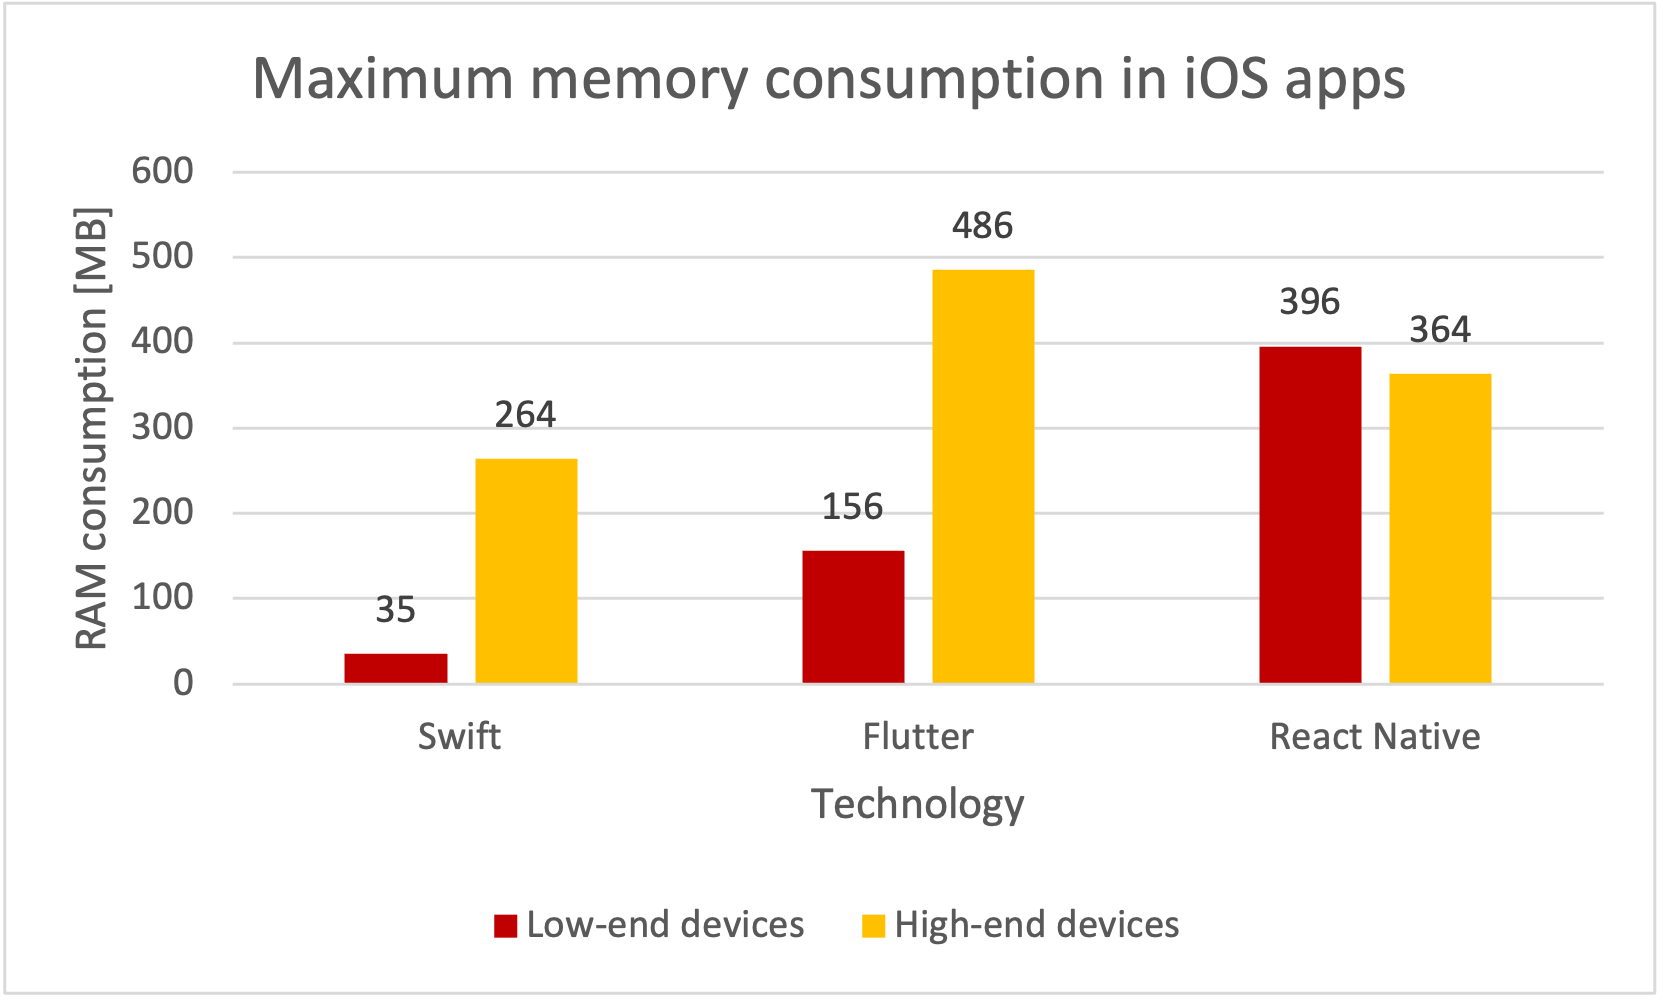
\includegraphics[width=\textwidth]{img/ram_max_ios}
        \caption{Maximum memory consumption in iOS apps (Source: Own work)}
        \label{fig:ram_max_ios}
    \end{minipage}
\end{figure}

Figures \ref{fig:ram_avg_ios} and \ref{fig:ram_max_ios} show the comparison of memory consumption among iOS apps developed with Swift, Flutter, and React Native. Swift apps exhibit considerably lower memory consumption compared to the other technologies. For low-end devices, Flutter performs moderately better than React Native. On the other hand, React Native apps utilize less memory on high-end devices than Flutter apps. Again, Flutter is responsible for the highest spikes on high-end devices.

\begin{figure}[H]
    \begin{minipage}{.48\textwidth}
        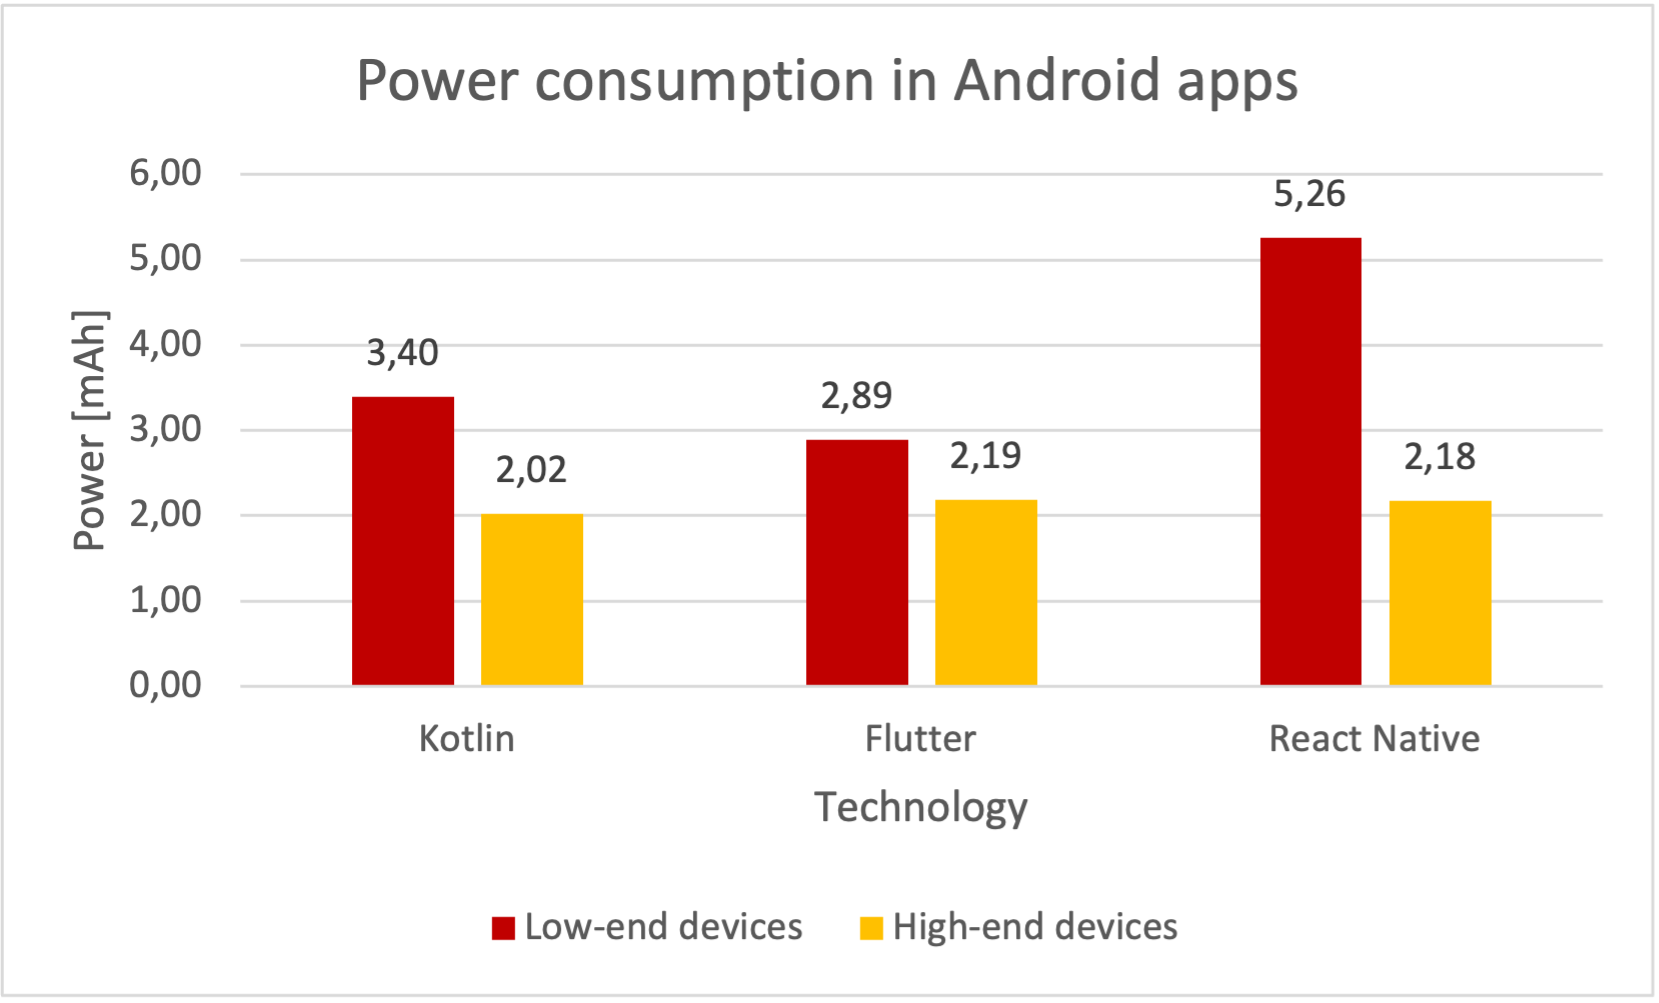
\includegraphics[width=\textwidth]{img/power_android}
        \caption{Power consumption in Android apps (Source: Own work)}
        \label{fig:power_android}
    \end{minipage}
    \hfill
    \begin{minipage}{.48\textwidth}
        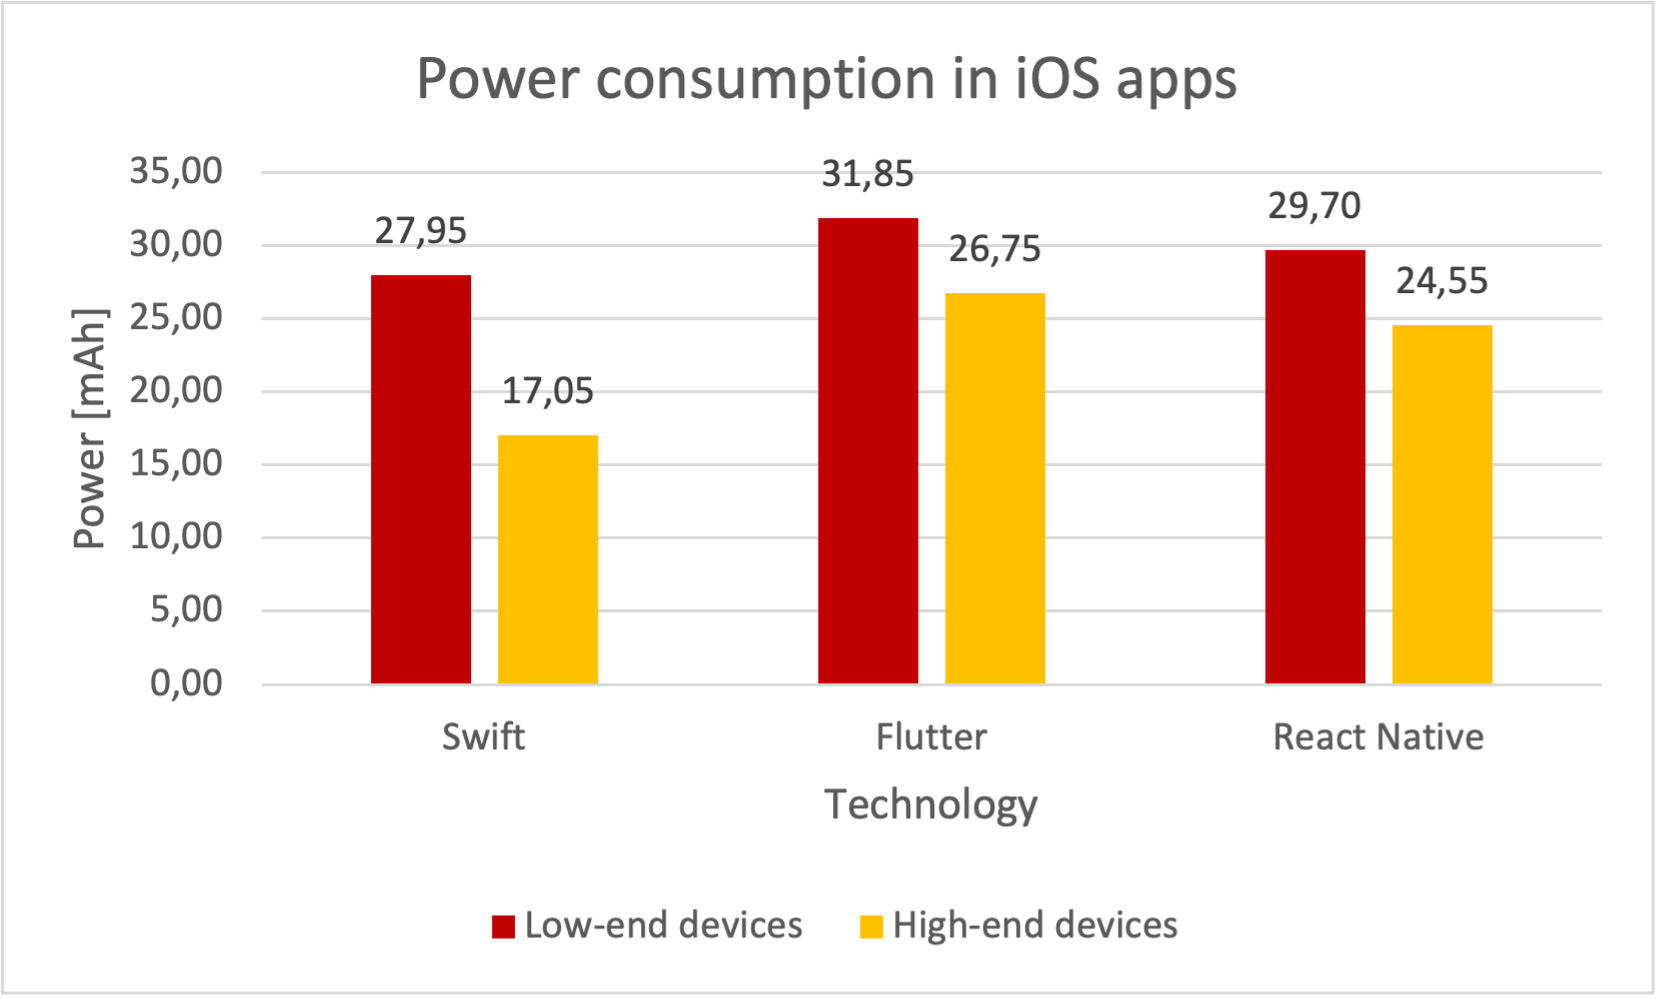
\includegraphics[width=\textwidth]{img/power_ios}
        \caption{Power consumption in iOS apps (Source: Own work)}
        \label{fig:power_ios}
    \end{minipage}
\end{figure}

Figures \ref{fig:power_android} and \ref{fig:power_ios} show the comparison of power consumption among Android and iOS apps developed with Kotlin, Flutter, Swift, and React Native. Overall, Android apps perform similarly on high-end devices. Considering power consumption on low-end devices, Flutter handles it the best. Although the values themselves are really low, the experiment was only carried out for a duration of one minute; therefore, with real-life usage, those values would be further apart. In the case of iOS apps, the results are quite close, apart from Swift apps that perform noticeably better on high-end devices.

\begin{figure}[H]
    \begin{minipage}{.48\textwidth}
        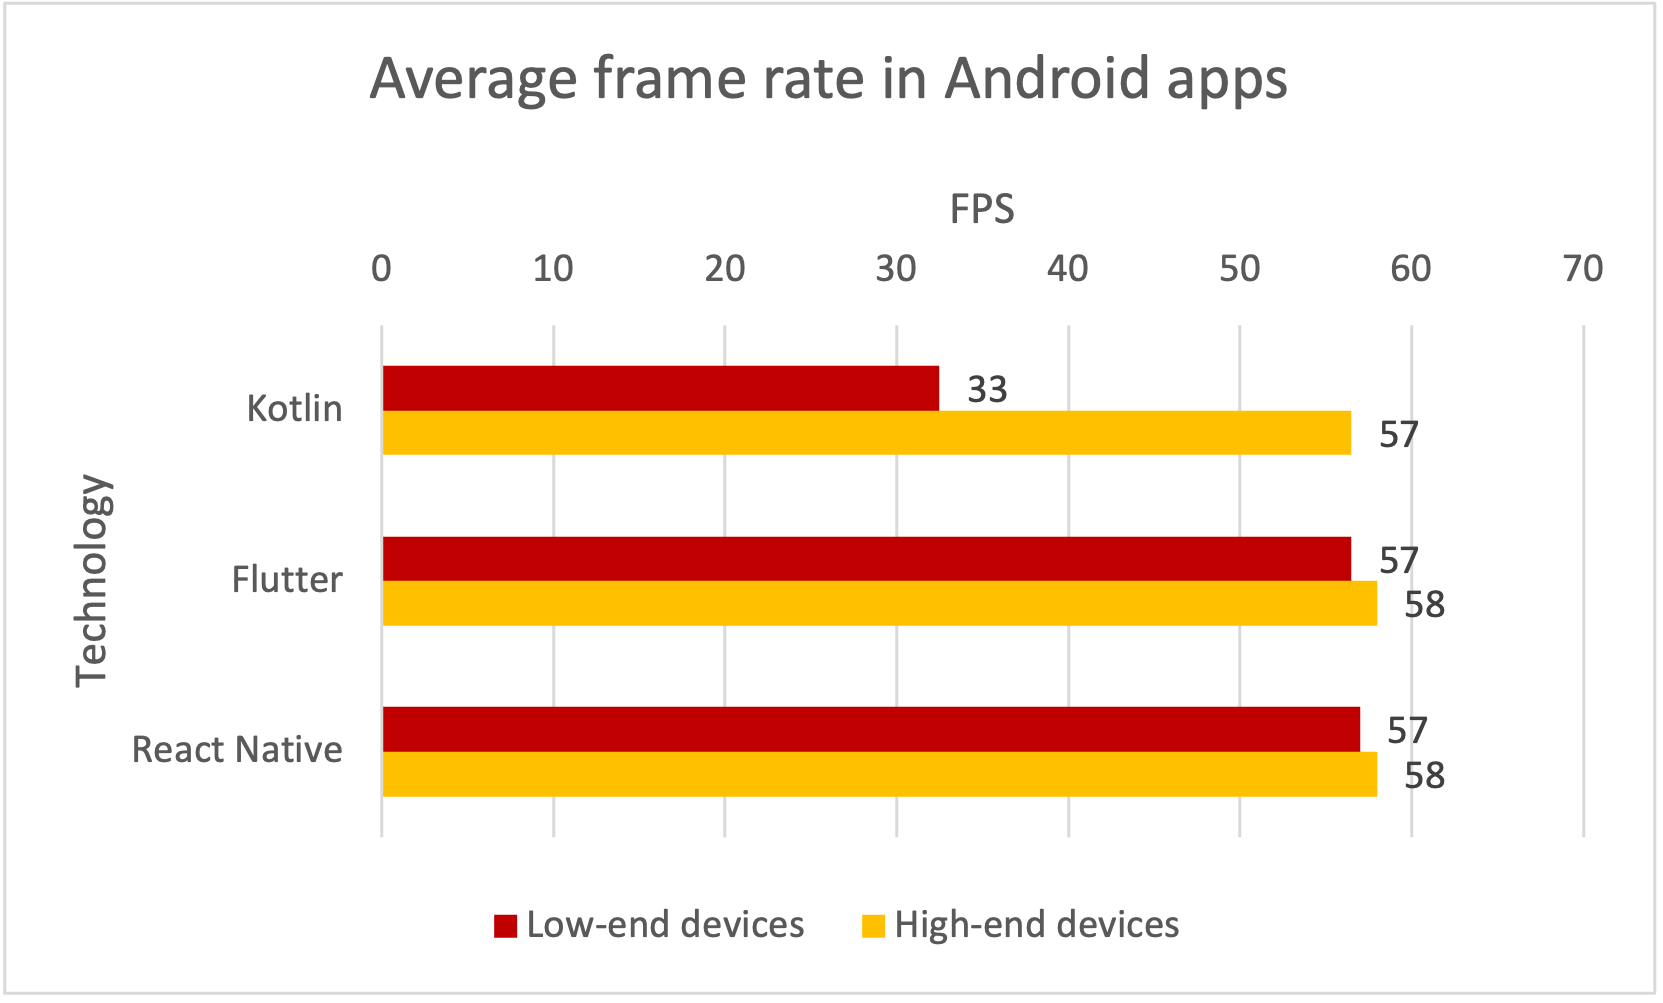
\includegraphics[width=\textwidth]{img/fps_average_android}
        \caption{Average frame rate in Android apps (Source: Own work)}
        \label{fig:fps_avg_android}
    \end{minipage}
    \hfill
    \begin{minipage}{.48\textwidth}
        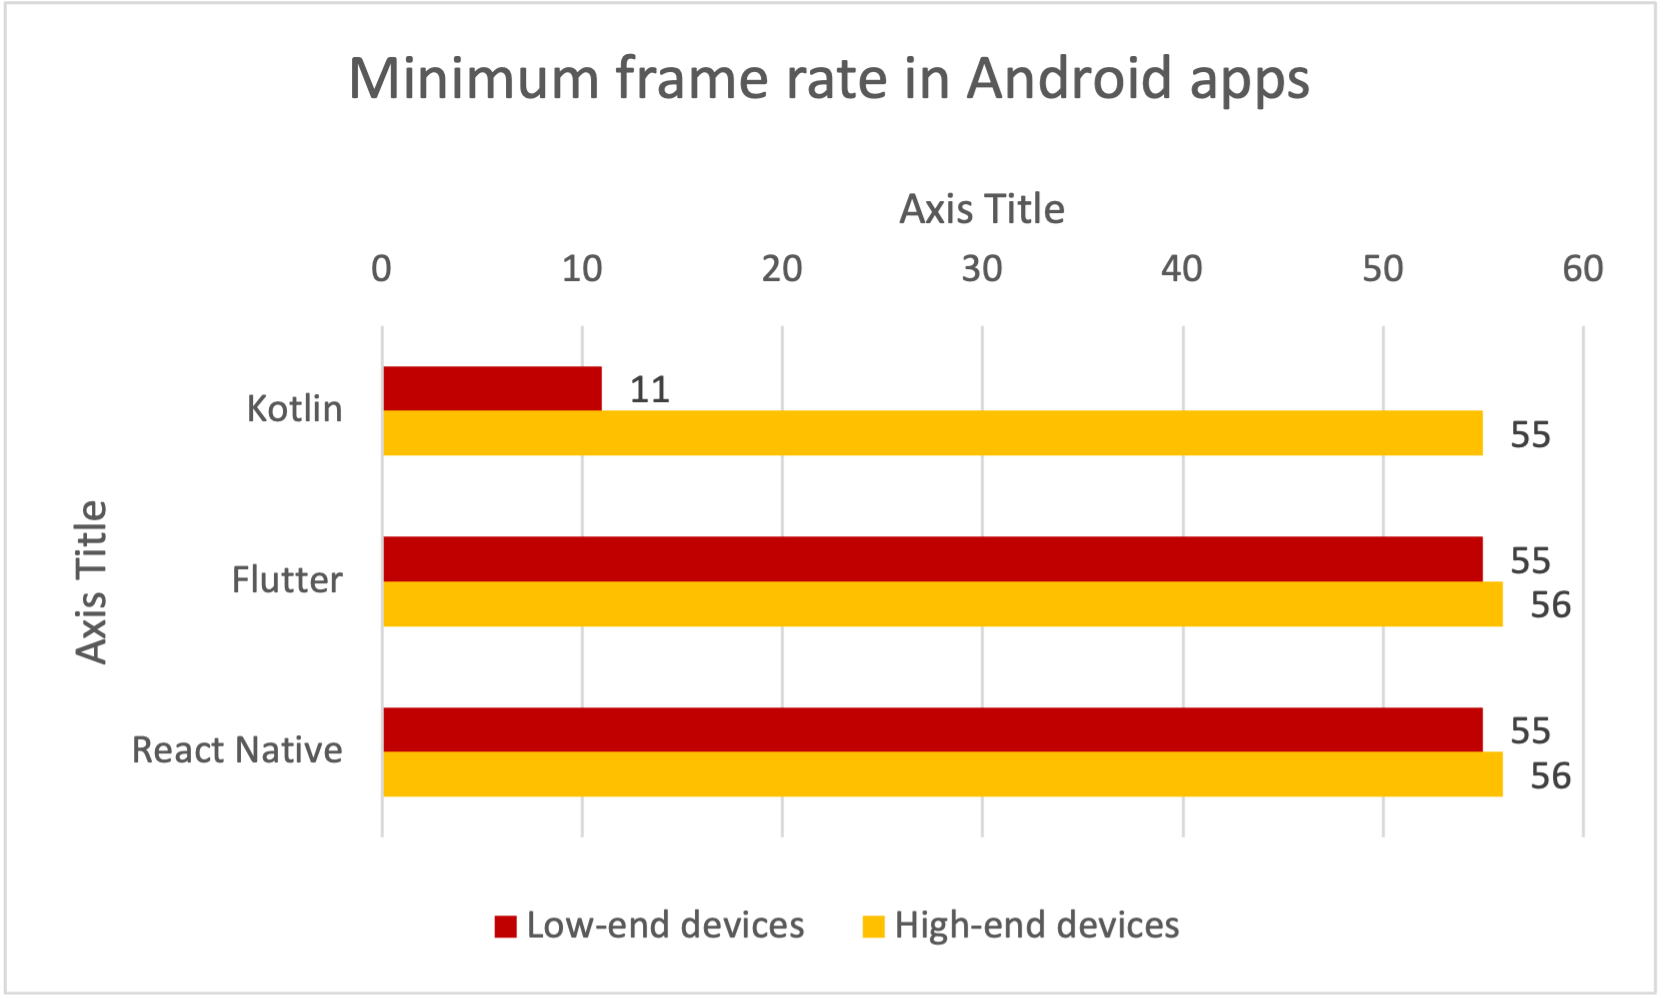
\includegraphics[width=\textwidth]{img/fps_min_android}
        \caption{Minimum frame rate in Android apps (Source: Own work)}
        \label{fig:fps_min_android}
    \end{minipage}
\end{figure}

Figures \ref{fig:fps_avg_android} and \ref{fig:fps_min_android} show the comparison of frame rate among Android apps developed with Kotlin, Flutter, and React Native. For high-end devices, there are no significant differences in the smoothness of apps developed with either technology. The range of 55--58 FPS on average is considered to be an excellent result. However, Kotlin apps struggle on low-end devices, experiencing 10 FPS drops and an average frame rate of 33 FPS. Flutter and React Native apps achieve similarly good results on low-end and high-end devices.

\begin{figure}[H]
    \begin{minipage}{.48\textwidth}
        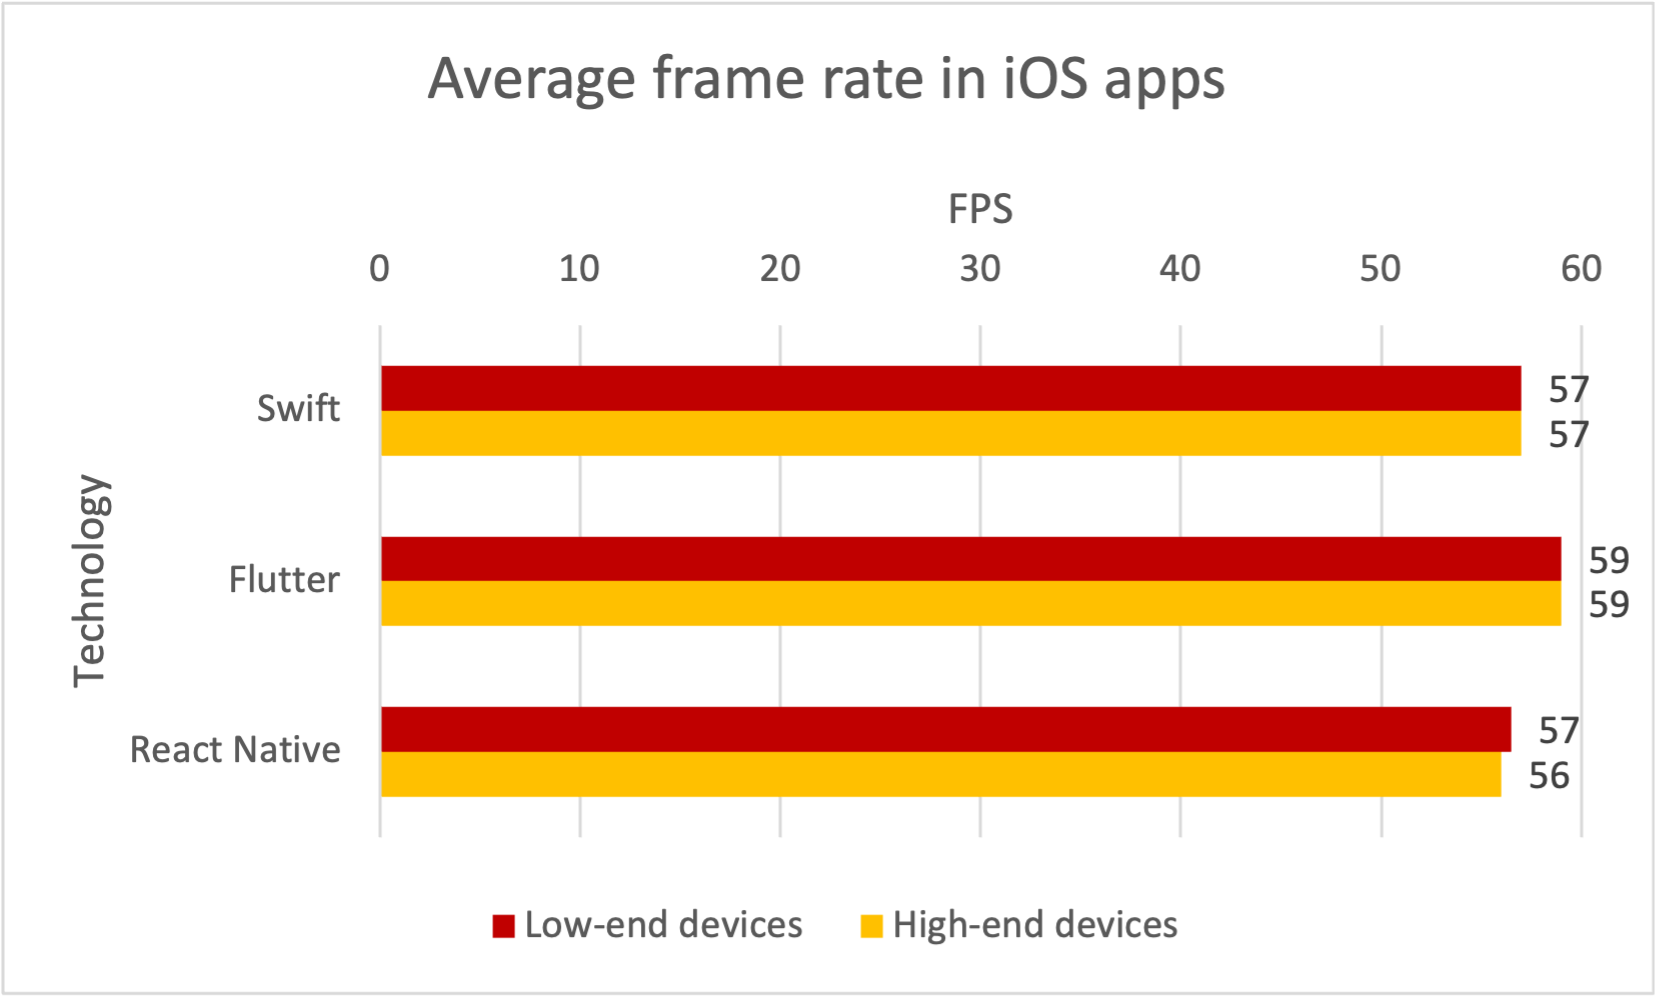
\includegraphics[width=\textwidth]{img/fps_average_ios}
        \caption{Average frame rate in iOS apps (Source: Own work)}
        \label{fig:fps_avg_ios}
    \end{minipage}
    \hfill
    \begin{minipage}{.48\textwidth}
        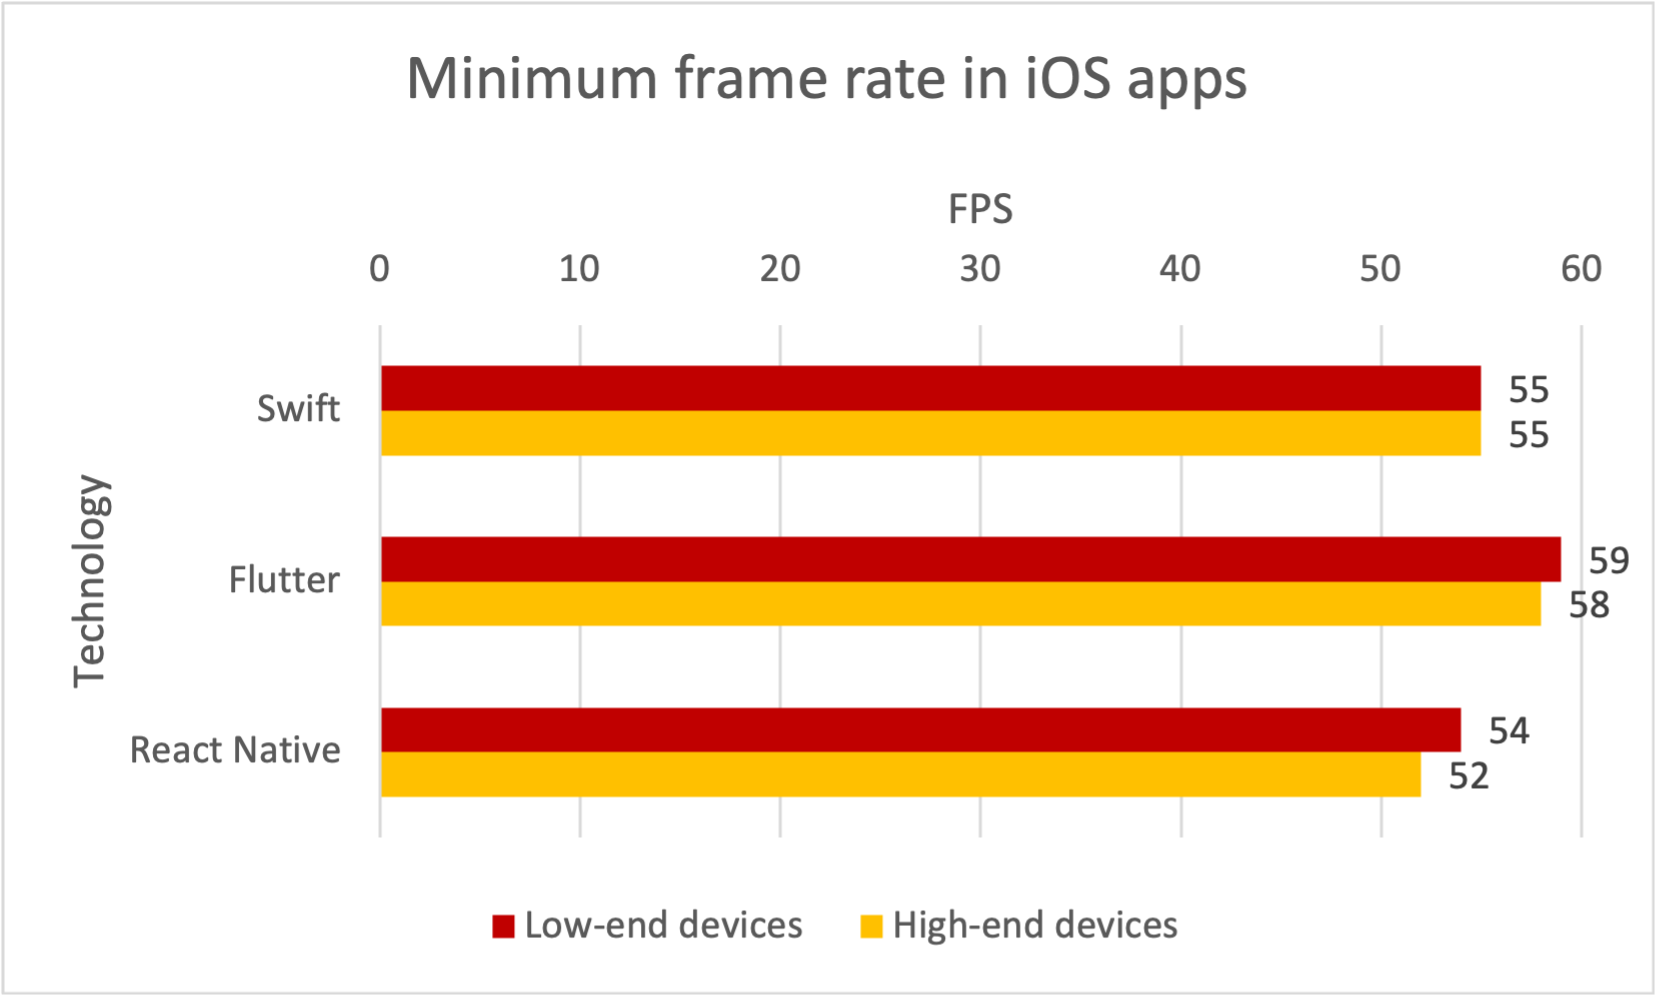
\includegraphics[width=\textwidth]{img/fps_min_ios}
        \caption{Minimum frame rate in iOS apps (Source: Own work)}
        \label{fig:fps_min_ios}
    \end{minipage}
\end{figure}

Figures \ref{fig:fps_avg_ios} and \ref{fig:fps_min_ios} show the comparison of frame rate among iOS apps developed with Swift, Flutter, and React Native. Overall, Flutter apps exhibit the highest frame rate of 59 FPS on low-end and high-end devices. Swift and React Native apps demonstrate 56--57 FPS frame rate on average. No significant FPS drops can be observed, with React Native apps experiencing a minimum of 52 FPS on high-end devices.

\begin{figure}[H]
    \begin{minipage}{.48\textwidth}
        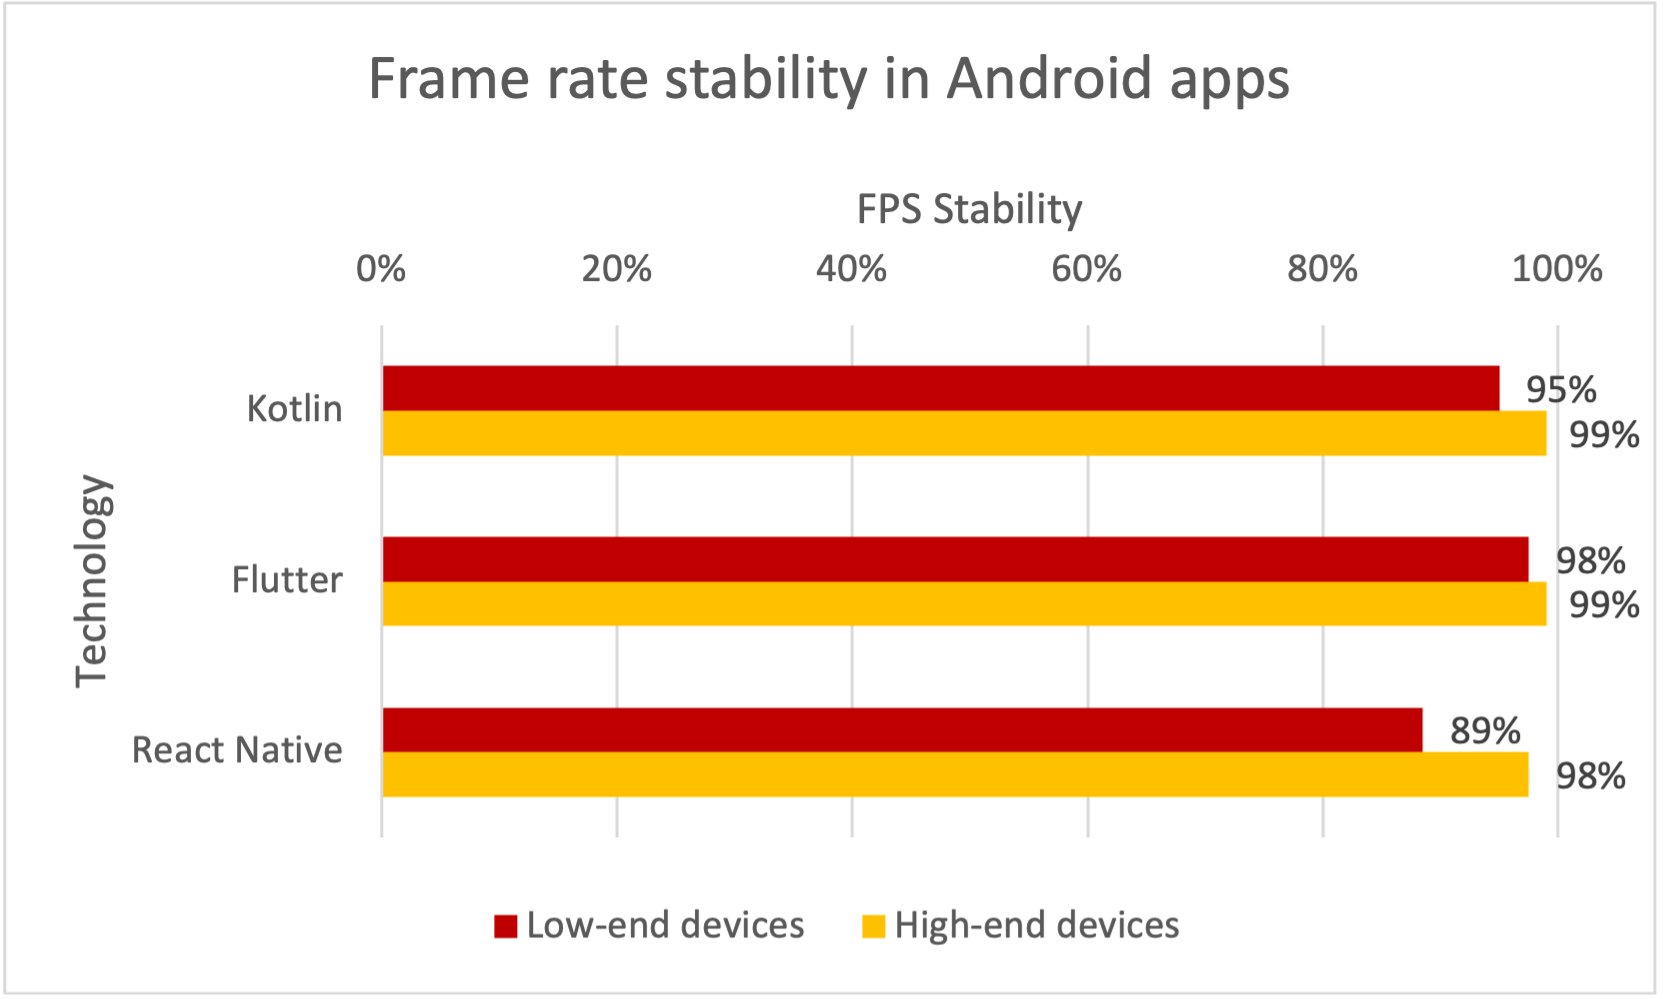
\includegraphics[width=\textwidth]{img/fps_stability_android}
        \caption{Frame rate stability in Android apps (Source: Own work)}
        \label{fig:fps_stability_android}
    \end{minipage}
    \hfill
    \begin{minipage}{.48\textwidth}
        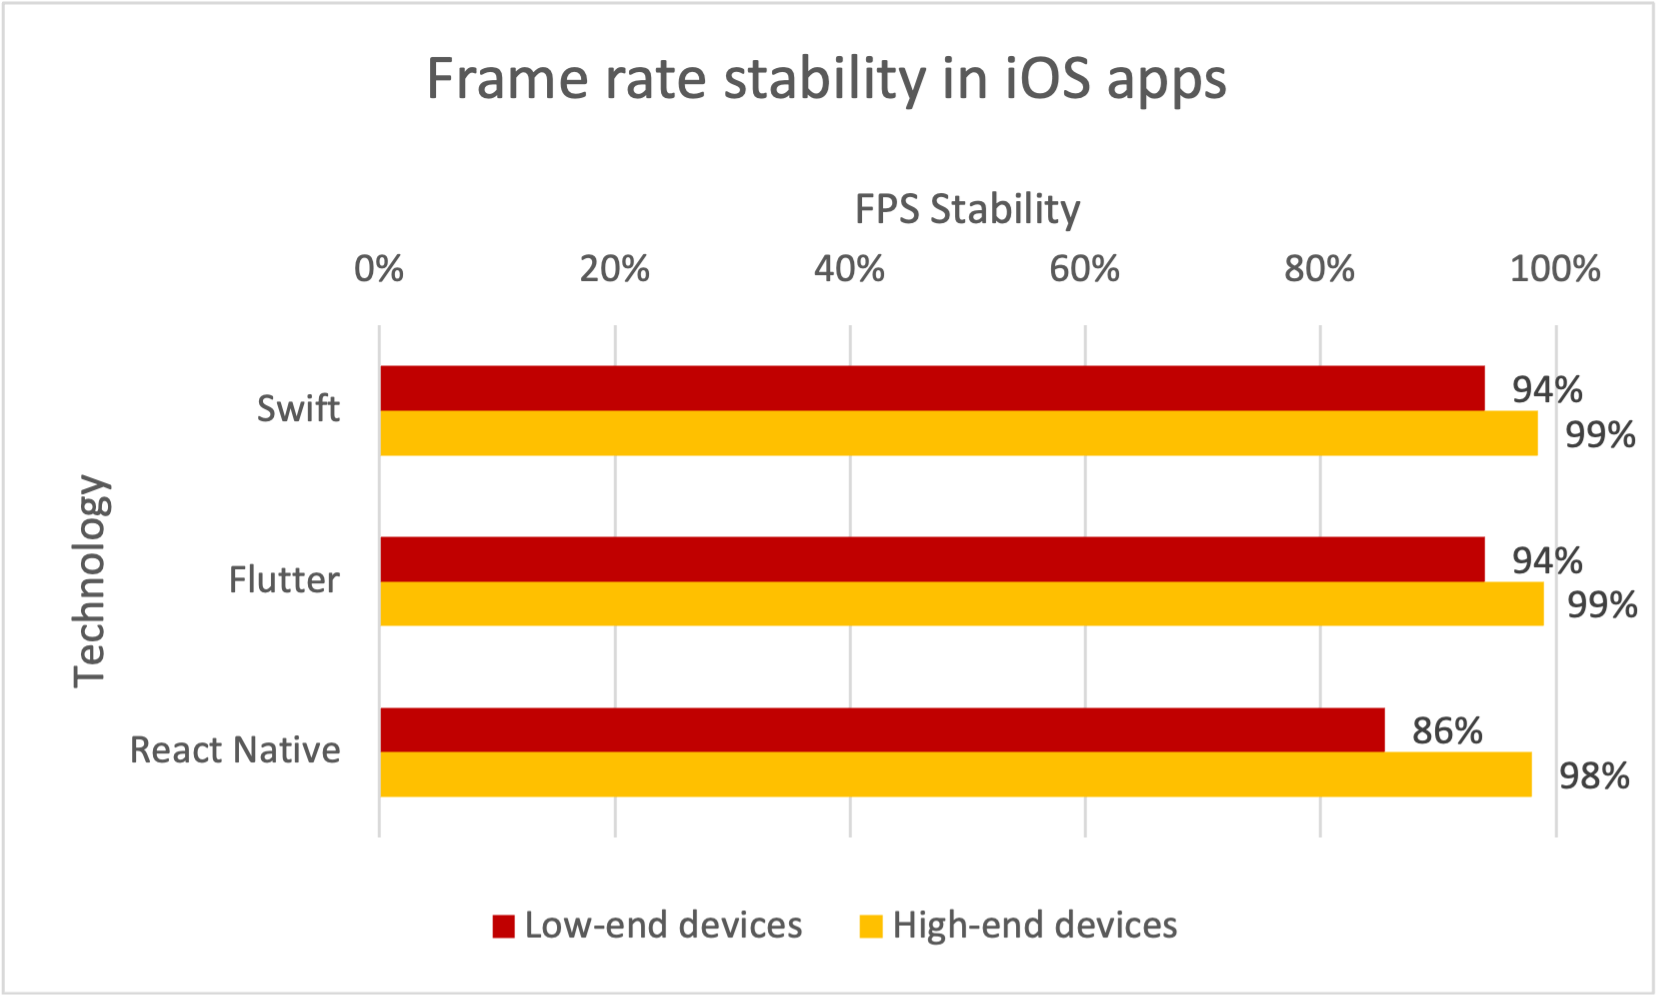
\includegraphics[width=\textwidth]{img/fps_stability_ios}
        \caption{Frame rate stability in iOS apps (Source: Own work)}
        \label{fig:fps_stability_ios}
    \end{minipage}
\end{figure}

Figures \ref{fig:fps_stability_android} and \ref{fig:fps_stability_ios} show the comparison of frame rate stability among Android and iOS apps developed with Kotlin, Swift, Flutter, and React Native. The results are closely comparable, considering either platform. On both low-end and high-end devices, each technology offers high frame rate stability. Only React Native apps installed on low-end devices experience stability below 90\%.


% !TEX encoding = UTF-8 Unicode 
% !TEX root = praca.tex

\subsection{Research scenario 1 results analysis}

The following figures illustrate the aggregated results from the experiments conducted within Research scenario 1 described in Chapter \ref{chap:research_scenarios}.

\begin{figure}[H]
    \begin{minipage}{.48\textwidth}
        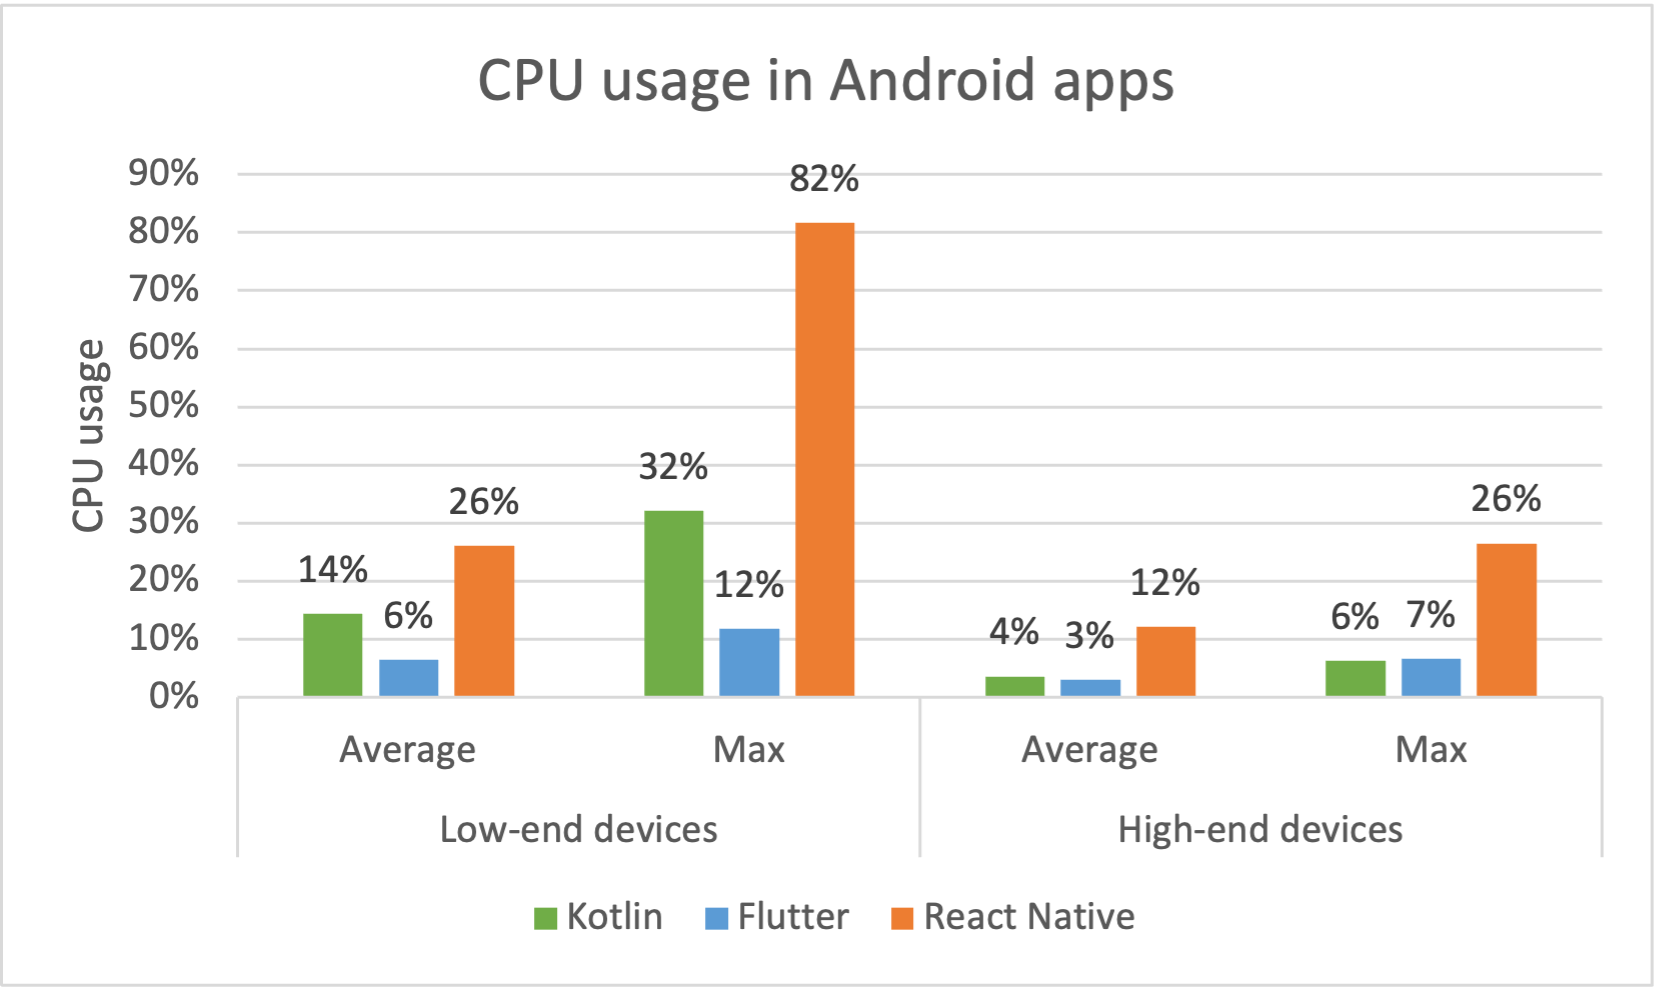
\includegraphics[width=\textwidth]{img/scenario1_cpu_android}
        \caption{Research scenario 1: CPU usage in Android apps (Source: Own work)}
        \label{fig:s1_cpu_android}
    \end{minipage}
    \hfill
    \begin{minipage}{.48\textwidth}
        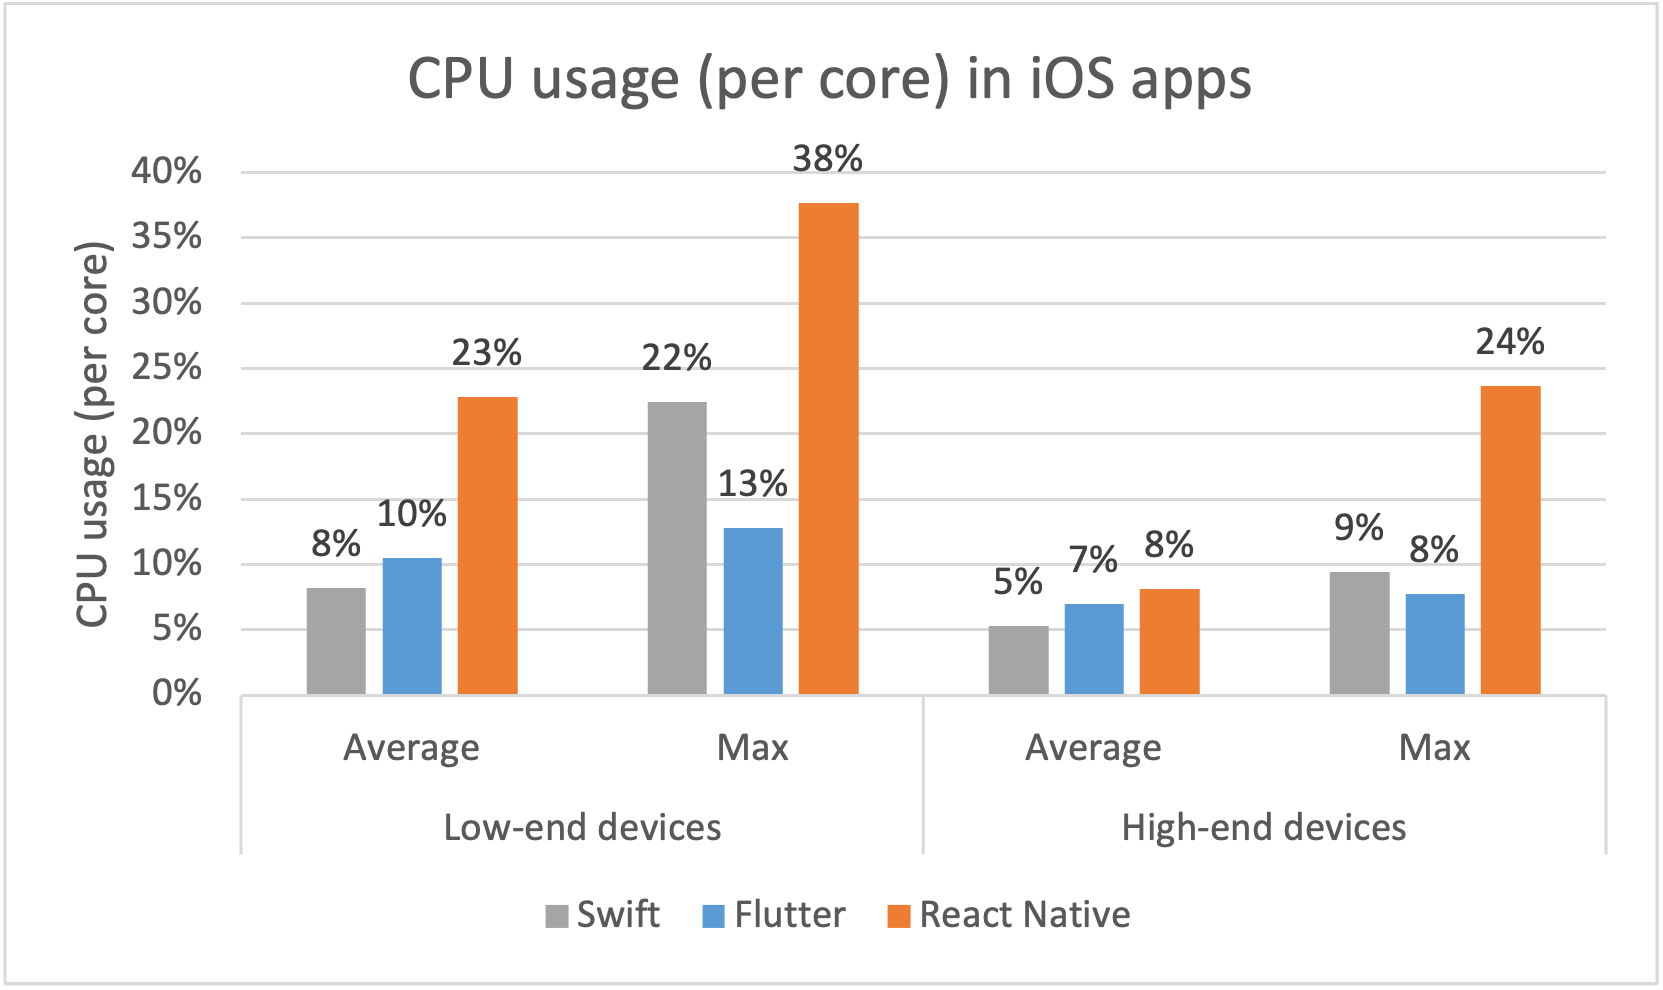
\includegraphics[width=\textwidth]{img/scenario1_cpu_ios}
        \caption{Research scenario 1: CPU usage in iOS apps (Source: Own work)}
        \label{fig:s1_cpu_ios}
    \end{minipage}
\end{figure}

Figures \ref{fig:s1_cpu_android} and \ref{fig:s1_cpu_ios} show the comparison of CPU usage among Android and iOS apps developed with Kotlin, Swift, Flutter, and React Native. For Android apps, Flutter offers the best performance, especially on low-end devices. Kotlin apps utilize 14\% of CPU capacity on average, which is almost two times less than React Native apps (26\%). React Native is again subject to the highest spikes, reaching a maximum of 82\% on low-end devices. On high-end devices, Flutter and Kotlin are on par, while React Native requires moderately more system resources. In the case of iOS apps, native apps developed with Swift demonstrate comparable CPU usage to Flutter apps on both low-end and high-end devices. Again, Flutter experiences the smallest spikes, while React Native exhibits the highest average CPU load combined with the most significant spikes.

\begin{figure}[H]
    \begin{minipage}{.48\textwidth}
        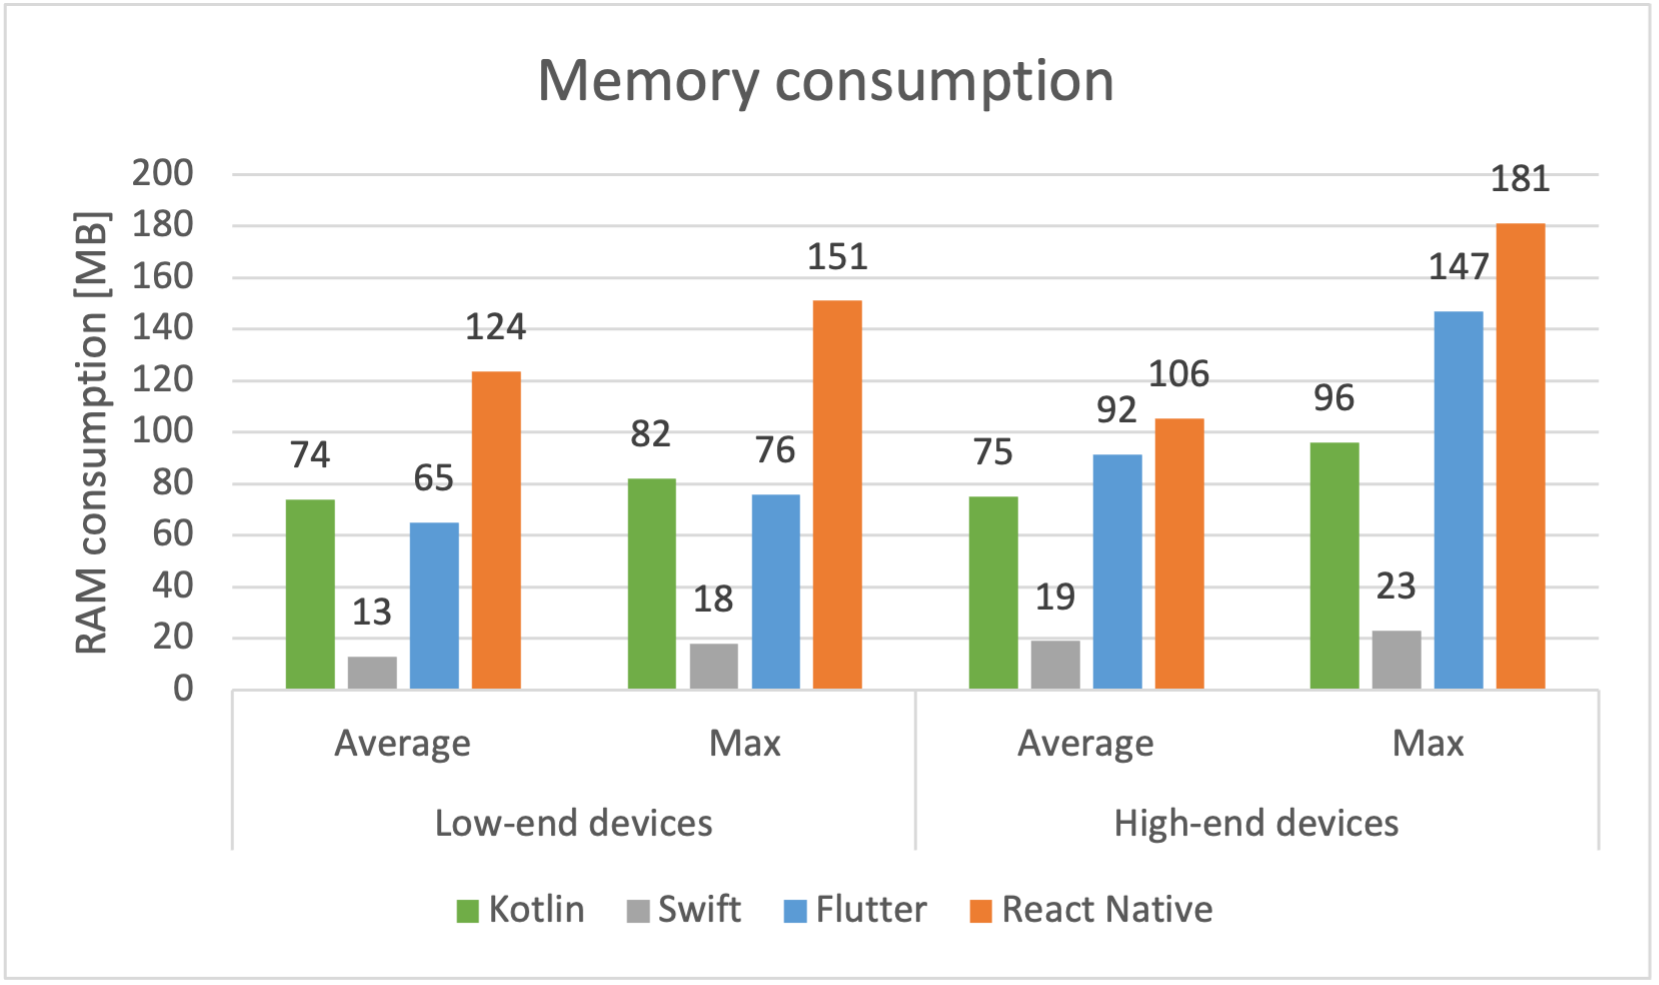
\includegraphics[width=\textwidth]{img/scenario1_ram}
    \caption{Research scenario 1: Memory consumption (Source: Own work)}
    \label{fig:s1_ram}
    \end{minipage}
    \hfill
    \begin{minipage}{.48\textwidth}
        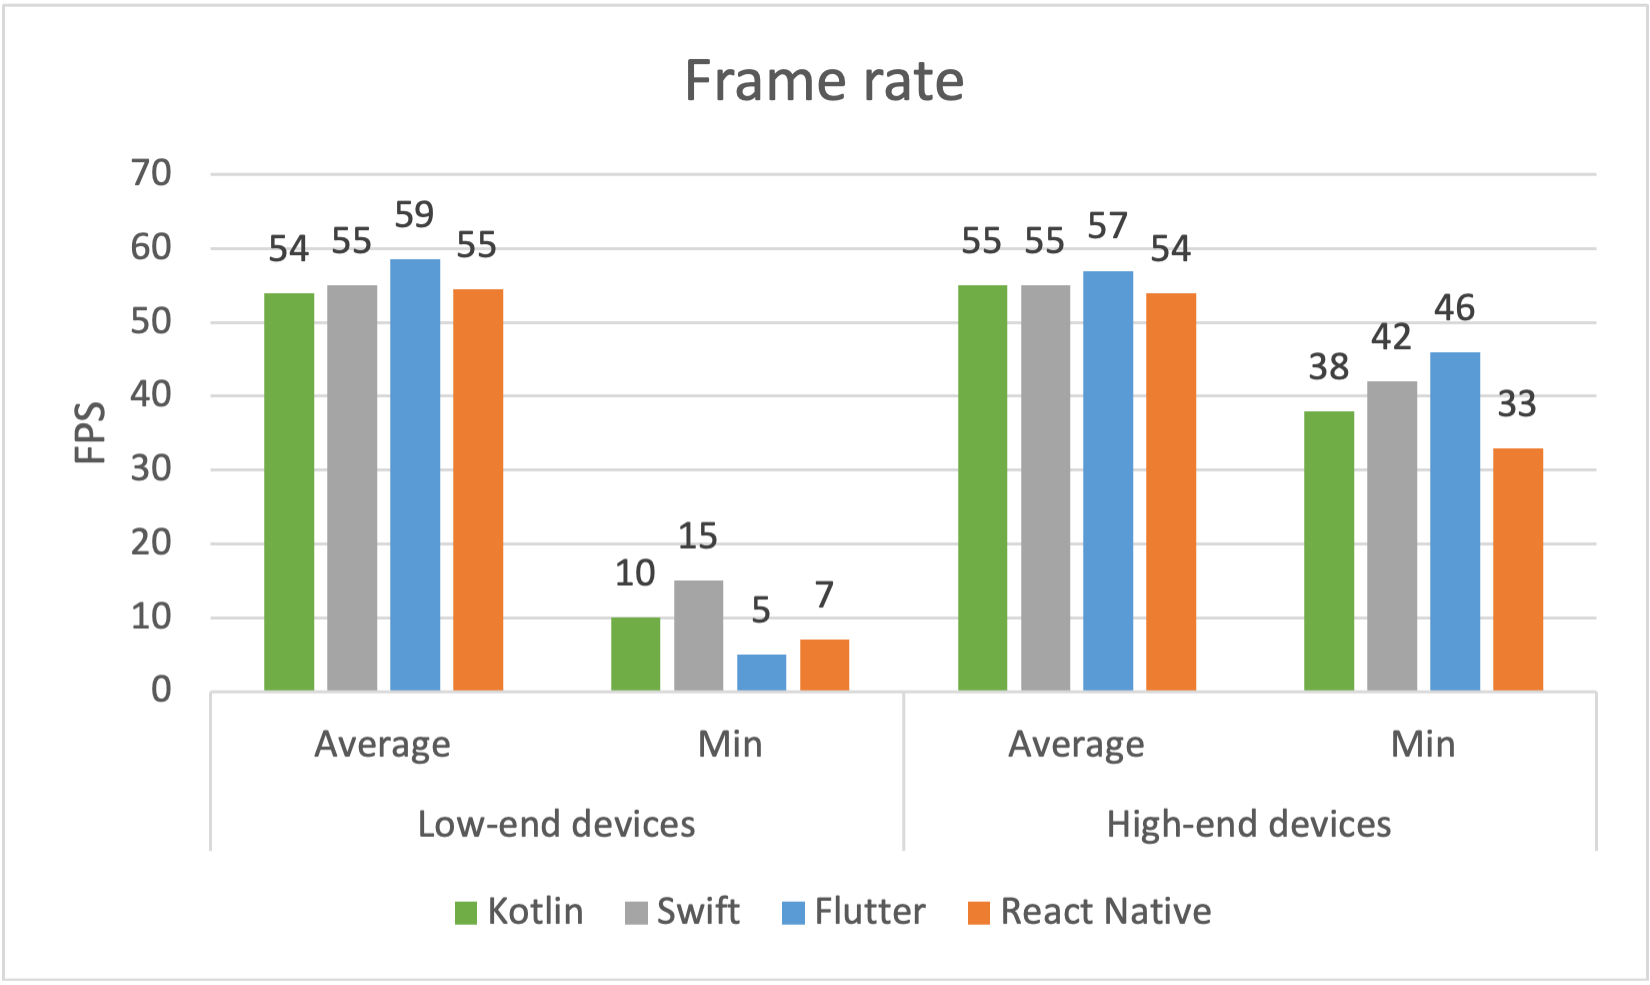
\includegraphics[width=\textwidth]{img/scenario1_fps}
    \caption{Research scenario 1: Frame rate (Source: Own work)}
    \label{fig:s1_fps}
    \end{minipage}
\end{figure}

Figure \ref{fig:s1_ram} shows the comparison of memory consumption among Android and iOS apps developed with Kotlin, Swift, Flutter, and React Native. It can be observed that Swift apps demonstrate the lowest memory consumption on all types of devices compared to other technologies. Flutter apps exhibit similar memory usage, with the latter experiencing higher spikes on high-end devices. React Native apps, on the other hand, perform moderately worse on low-end devices, slightly worse on high-end devices and suffer from bigger spikes.

\bigskip

Figure \ref{fig:s1_fps} show the comparison of frame rate among Android and iOS apps developed with Kotlin, Swift, Flutter, and React Native. In general, none of the technologies suffer from low frame rate on average. However, all of them experience sporadic FPS drops to as little as 5 FPS on low-end devices. Flutter seems to offer the highest overall smoothness with the best result on average and the highest minimum of 46 FPS on high-end devices.


% !TEX encoding = UTF-8 Unicode 
% !TEX root = praca.tex

\subsection{Research scenario 2 results analysis}

The following figures illustrate the aggregated results from the experiments conducted within Research scenario 2 described in Chapter \ref{chap:research_scenarios}.

\begin{figure}[H]
    \begin{minipage}{.48\textwidth}
        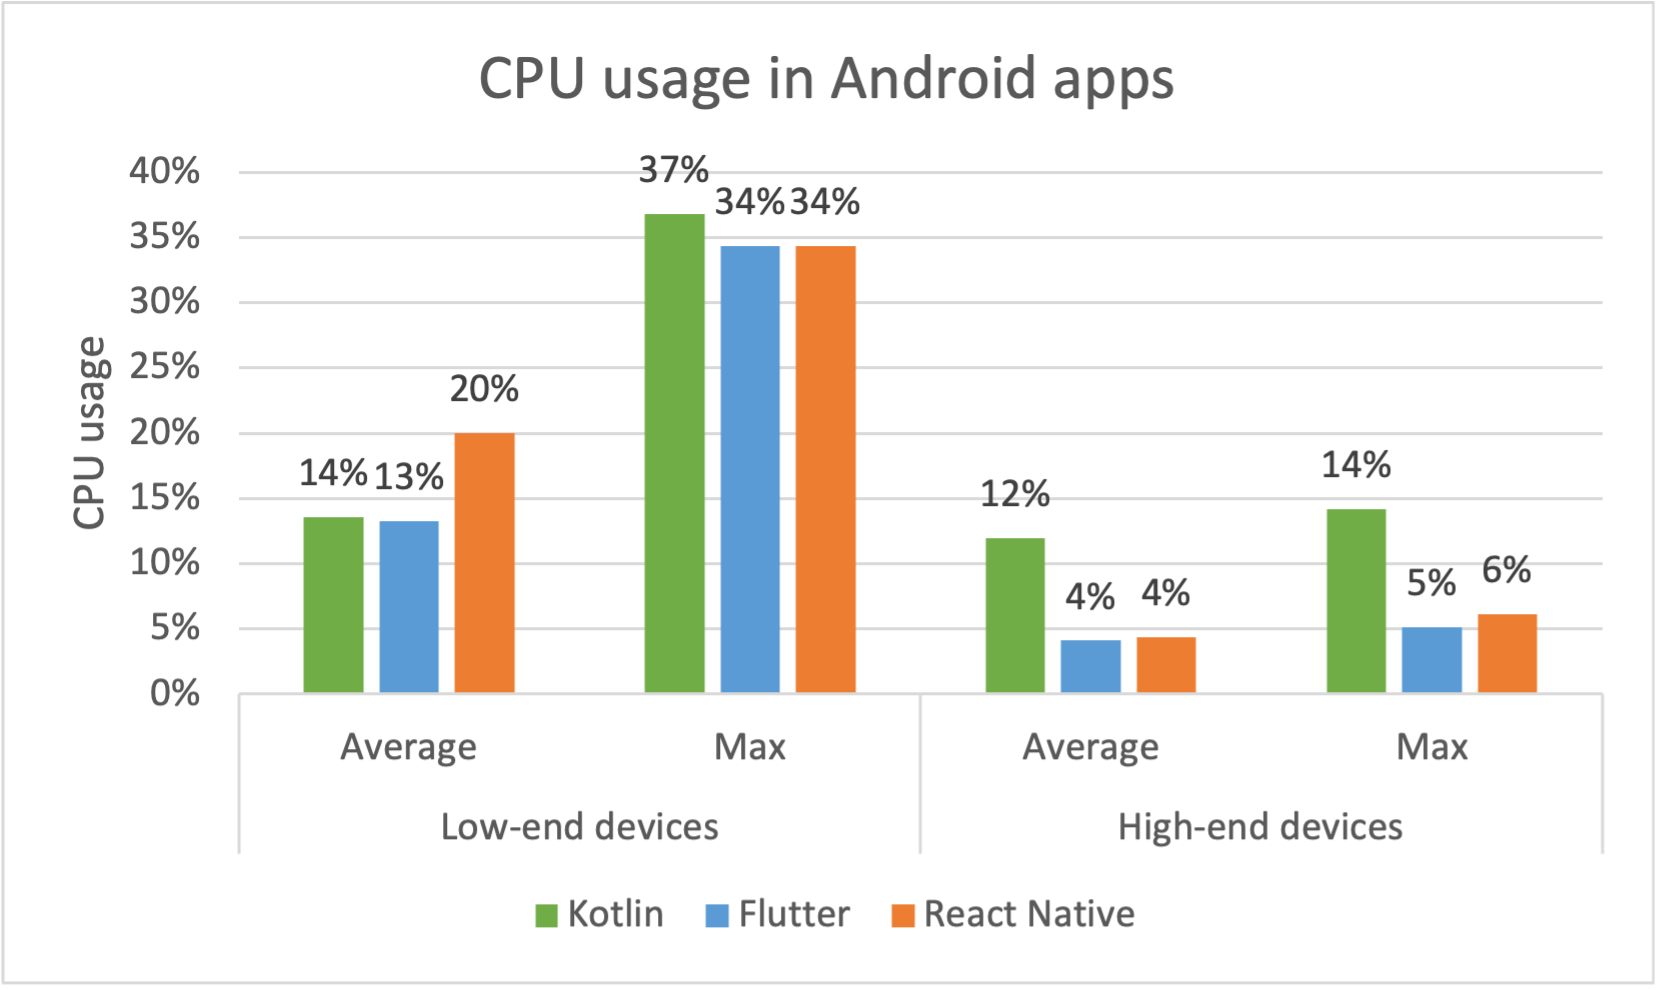
\includegraphics[width=\textwidth]{img/scenario2_cpu_android}
        \caption{Research scenario 2: CPU usage in Android apps (Source: Own work)}
        \label{fig:s2_cpu_android}
    \end{minipage}
    \hfill
    \begin{minipage}{.48\textwidth}
        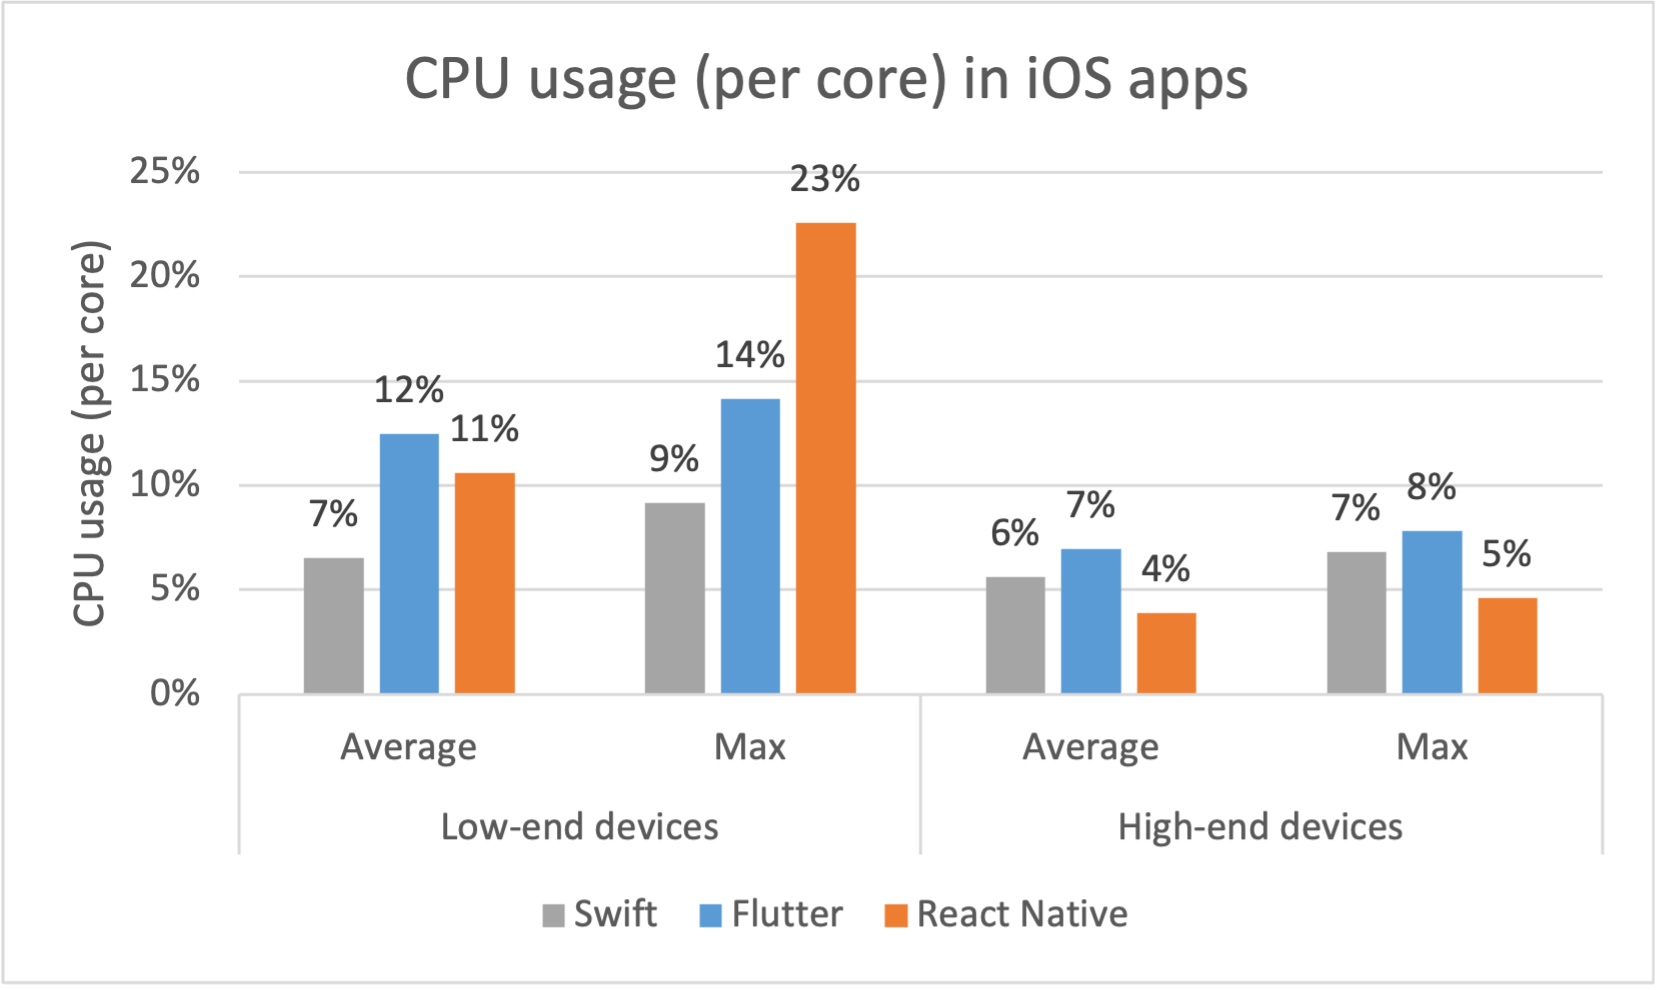
\includegraphics[width=\textwidth]{img/scenario2_cpu_ios}
        \caption{Research scenario 2: CPU usage in iOS apps (Source: Own work)}
        \label{fig:s2_cpu_ios}
    \end{minipage}
\end{figure}

Figures \ref{fig:s2_cpu_android} and \ref{fig:s2_cpu_ios} show the comparison of CPU usage among Android and iOS apps developed with Kotlin, Swift, Flutter, and React Native. In the case of Android apps, on lower-end devices, Kotlin and Flutter apps perform similarly, while React Native apps require slightly more CPU resources. However, on high-end devices, Flutter and React Native apps exhibit very low CPU usage and visibly outperform Kotlin apps. Swift apps running on low-end devices require the least CPU capacity, 7\% on average. Flutter and React Native apps exhibit similar CPU loads; however, the latter experience higher spikes. On high-end devices, all three technologies offer excellent performance while keeping CPU load within the threshold of 4--8\%.

\begin{figure}[H]
    \begin{minipage}{.48\textwidth}
        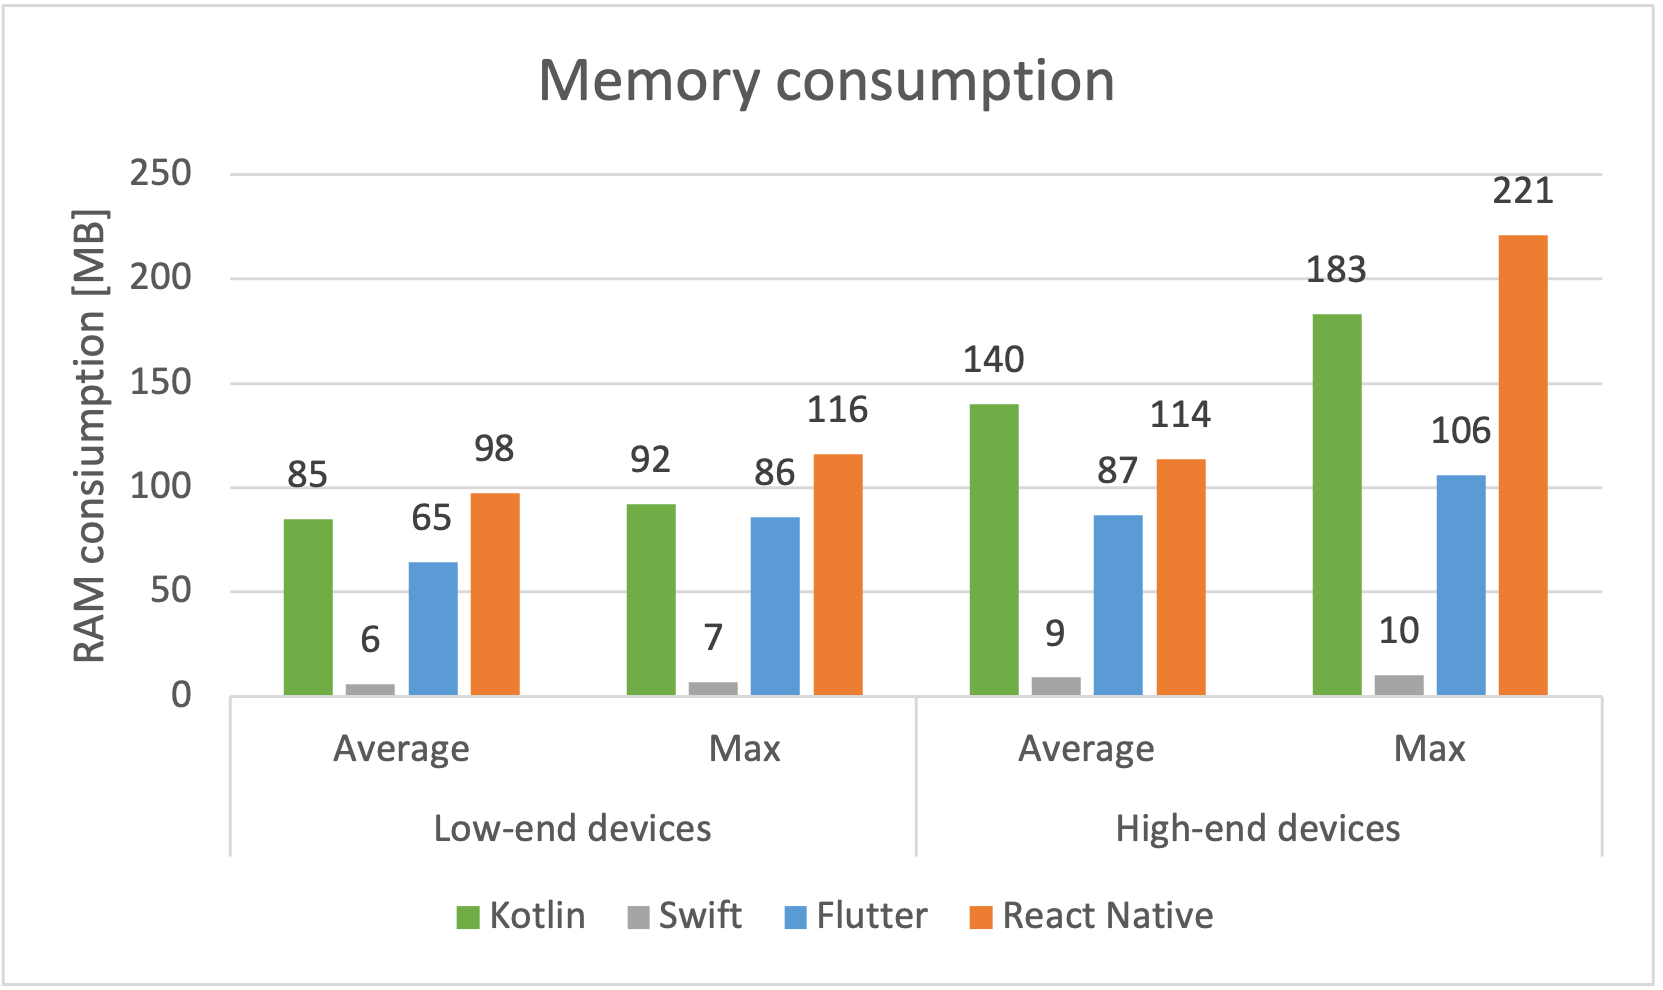
\includegraphics[width=\textwidth]{img/scenario2_ram}
        \caption{Research scenario 2: Memory consumption (Source: Own work)}
        \label{fig:s2_ram}
    \end{minipage}
    \hfill
    \begin{minipage}{.48\textwidth}
        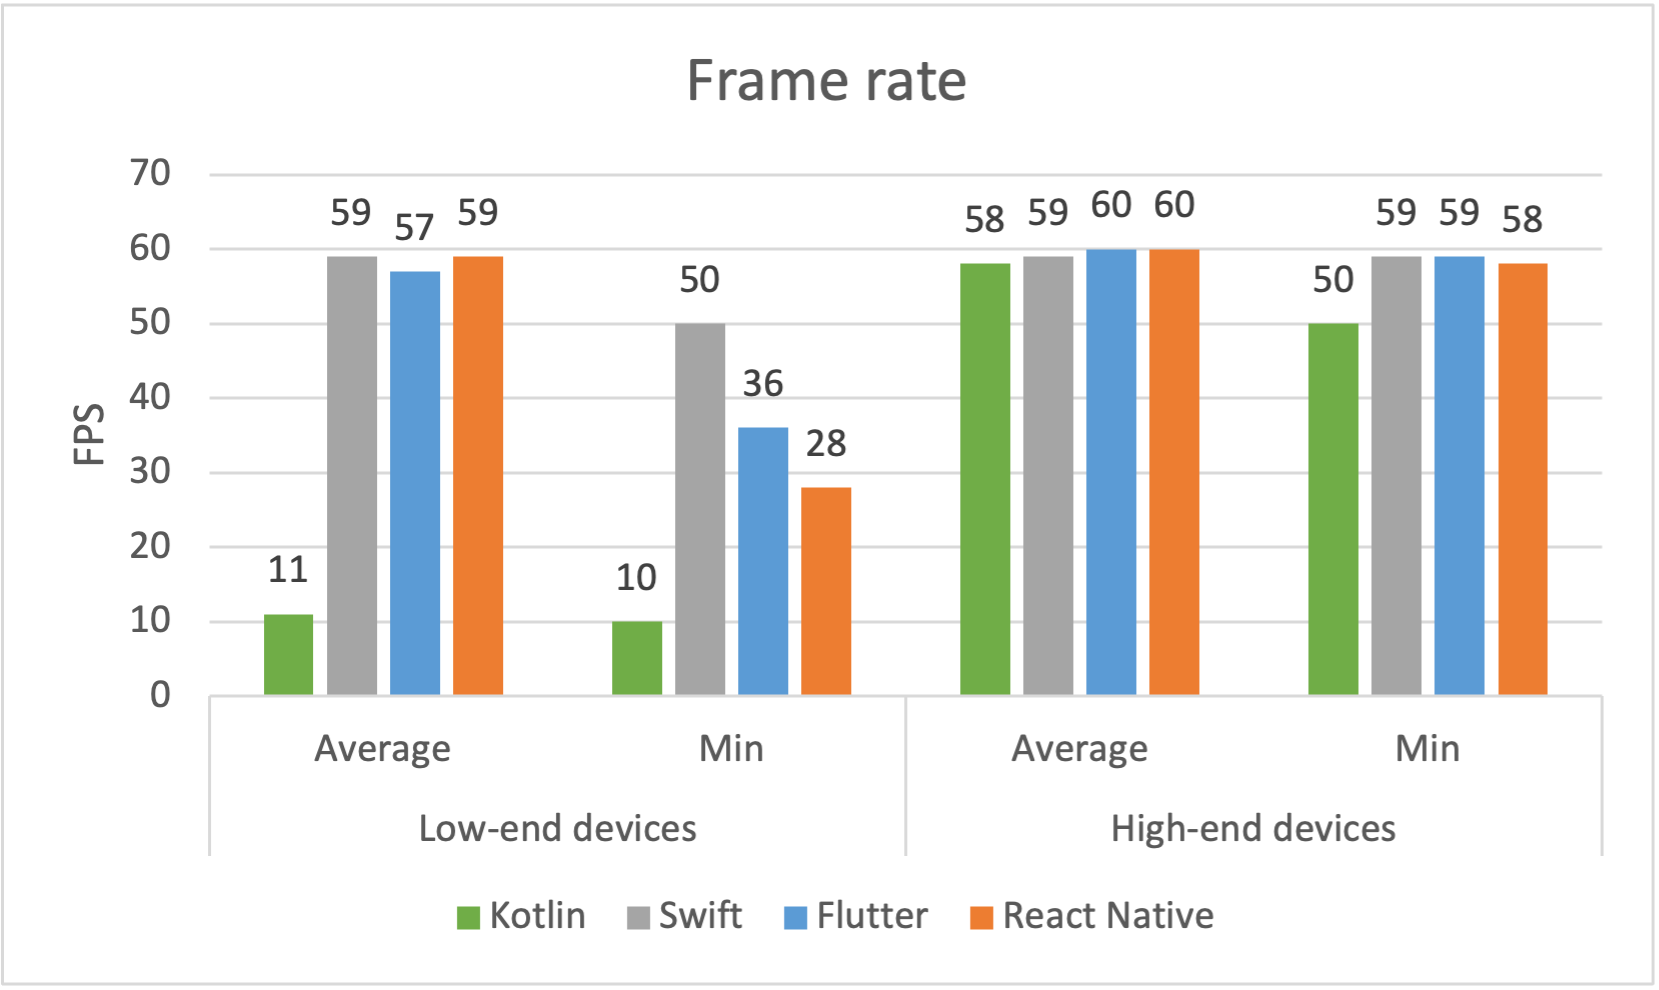
\includegraphics[width=\textwidth]{img/scenario2_fps}
    \caption{Research scenario 2: Frame rate (Source: Own work)}
    \label{fig:s2_fps}
    \end{minipage}
\end{figure}

Figure \ref{fig:s2_ram} shows the comparison of memory consumption among Android and iOS apps developed with Kotlin, Swift, Flutter, and React Native. Swift apps again demonstrate extremely low memory usage compared to other technologies and do not experience any spikes. Flutter apps slightly outperform Kotlin and React Native apps. Kotlin and React Native apps results are rather comparable. The former utilize less memory on low-end devices, and the latter require less memory on high-end devices, although they still experience higher spikes.

\bigskip

Figure \ref{fig:s2_fps} shows the comparison of frame rate among Android and iOS apps developed with Kotlin, Swift, Flutter, and React Native. On high-end devices, each technology exhibits similar performance, maintaining 58--FPS on average. Kotlin apps experience the biggest FPS drops; however, a minimum of 50 FPS is still not a concerning result. On low-end devices, Swift, Flutter, and React Native offer the same great performance, while Kotlin apps seem to suffer from a very low average frame rate of 11\%. Such a result corresponds to users experiencing visible stutters and lags. 

\clearpage


% !TEX encoding = UTF-8 Unicode 
% !TEX root = praca.tex

\subsection{Research scenario 3 results analysis}

The following figures illustrate the aggregated results from the experiments conducted within Research scenario 3 described in Chapter \ref{chap:research_scenarios}.

\begin{figure}[H]
    \begin{minipage}{.48\textwidth}
        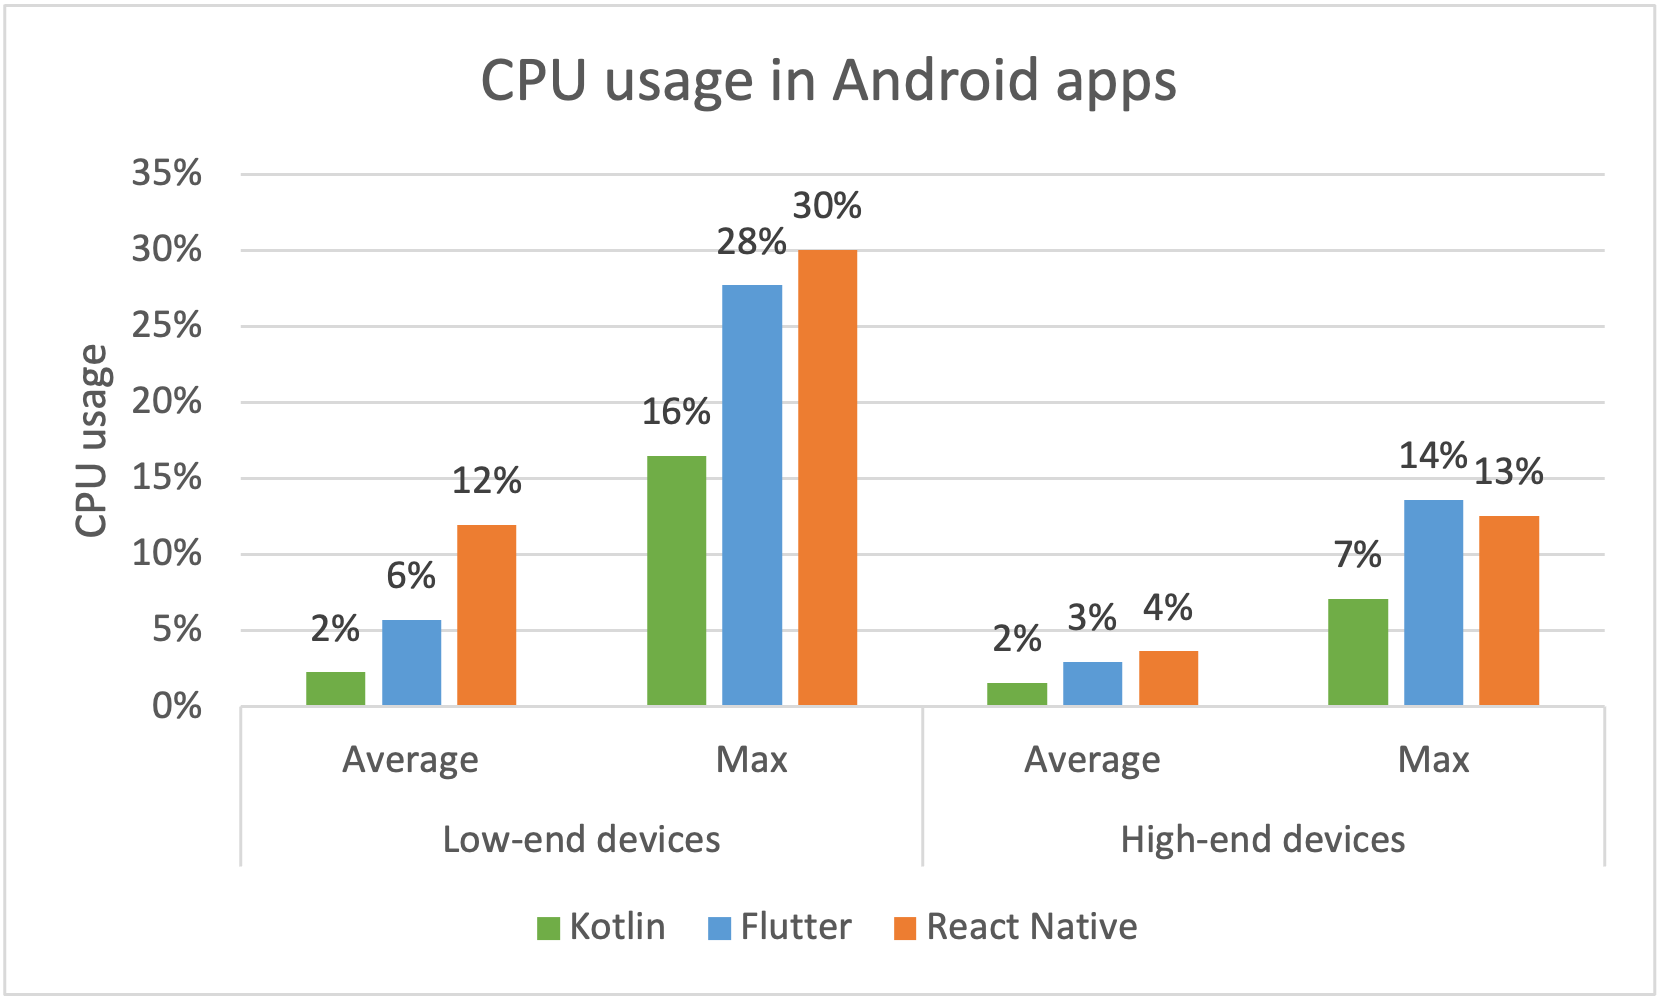
\includegraphics[width=\textwidth]{img/scenario3_cpu_android}
        \caption{Research scenario 3: CPU usage in Android apps (Source: Own work)}
        \label{fig:s3_cpu_android}
    \end{minipage}
    \hfill
    \begin{minipage}{.48\textwidth}
        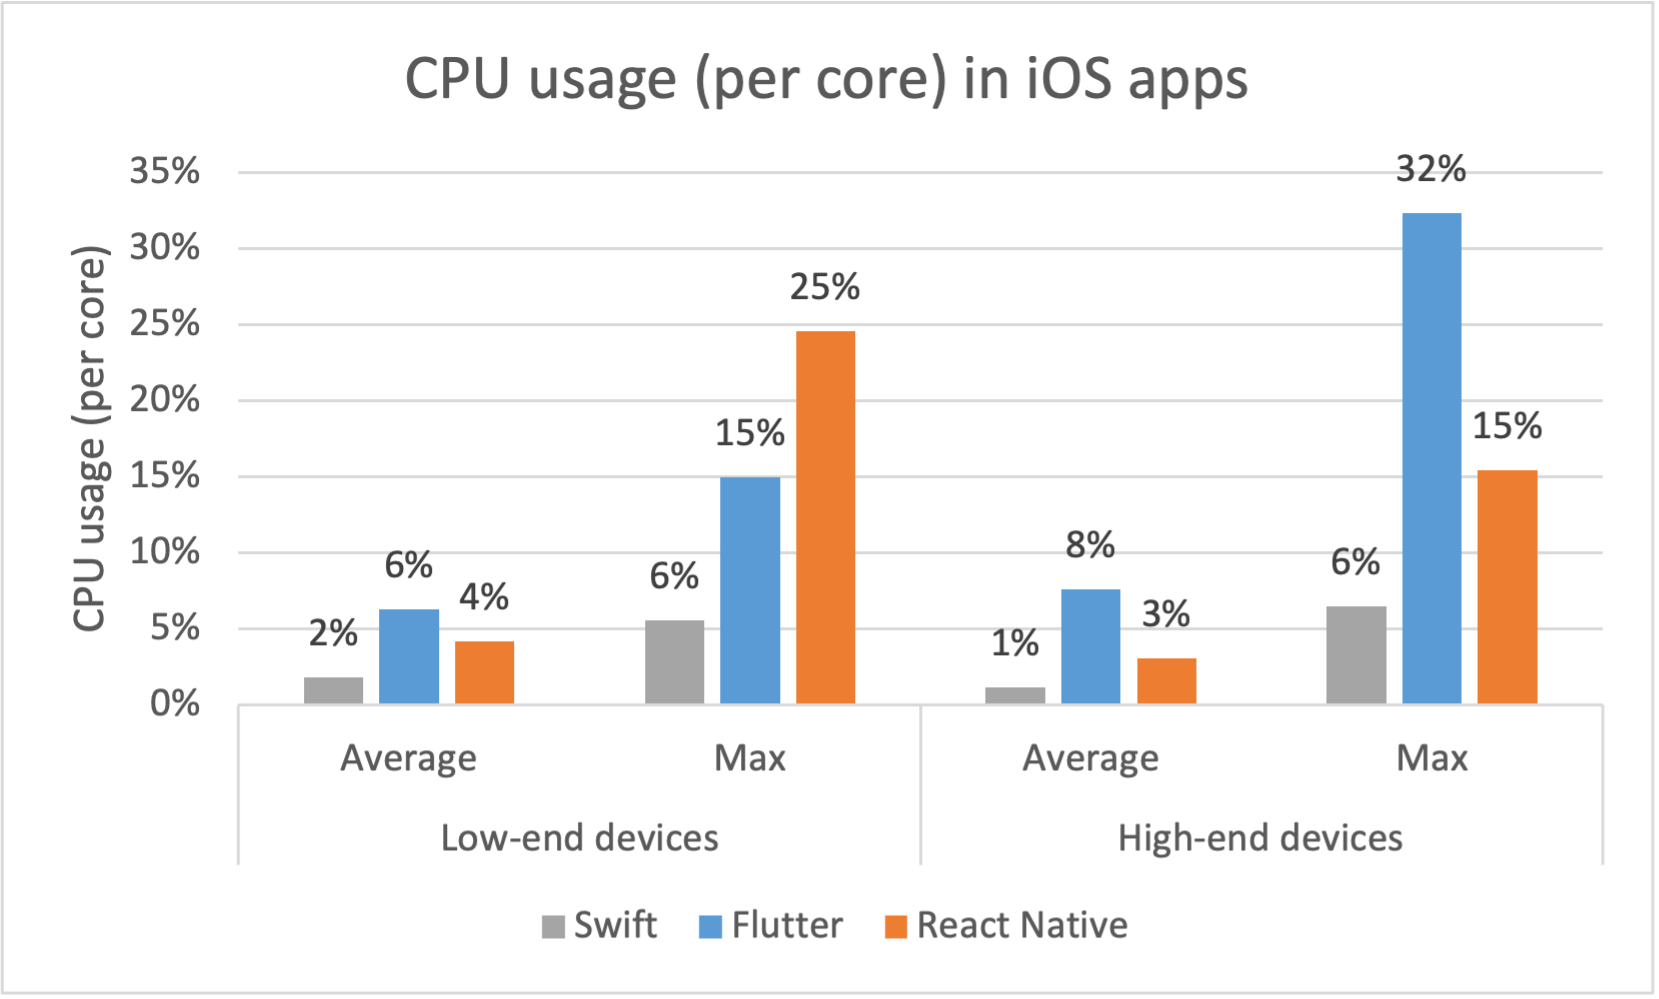
\includegraphics[width=\textwidth]{img/scenario3_cpu_ios}
        \caption{Research scenario 3: CPU usage in iOS apps (Source: Own work)}
        \label{fig:s3_cpu_ios}
    \end{minipage}
\end{figure}

Figures \ref{fig:s3_cpu_android} and \ref{fig:s3_cpu_ios} show the comparison of CPU usage among Android and iOS apps developed with Kotlin, Swift, Flutter, and React Native. On low-end and high-end Android devices, Kotlin apps provide the best performance at 2\% CPU load, followed by Flutter apps at 3--6\% and finally React Native apps at 4-12\%. When it comes to maximums reached, Flutter and React Native are again outperformed by Kotlin, but the values themselves are still relatively low. In the case of iOS, Swift apps show the lowest CPU load as well as no spikes on both low-end and high-end devices. React Native apps demonstrate slightly lower CPU usage than Flutter apps, although they experience higher spikes on low-end devices.

\begin{figure}[H]
    \centering
    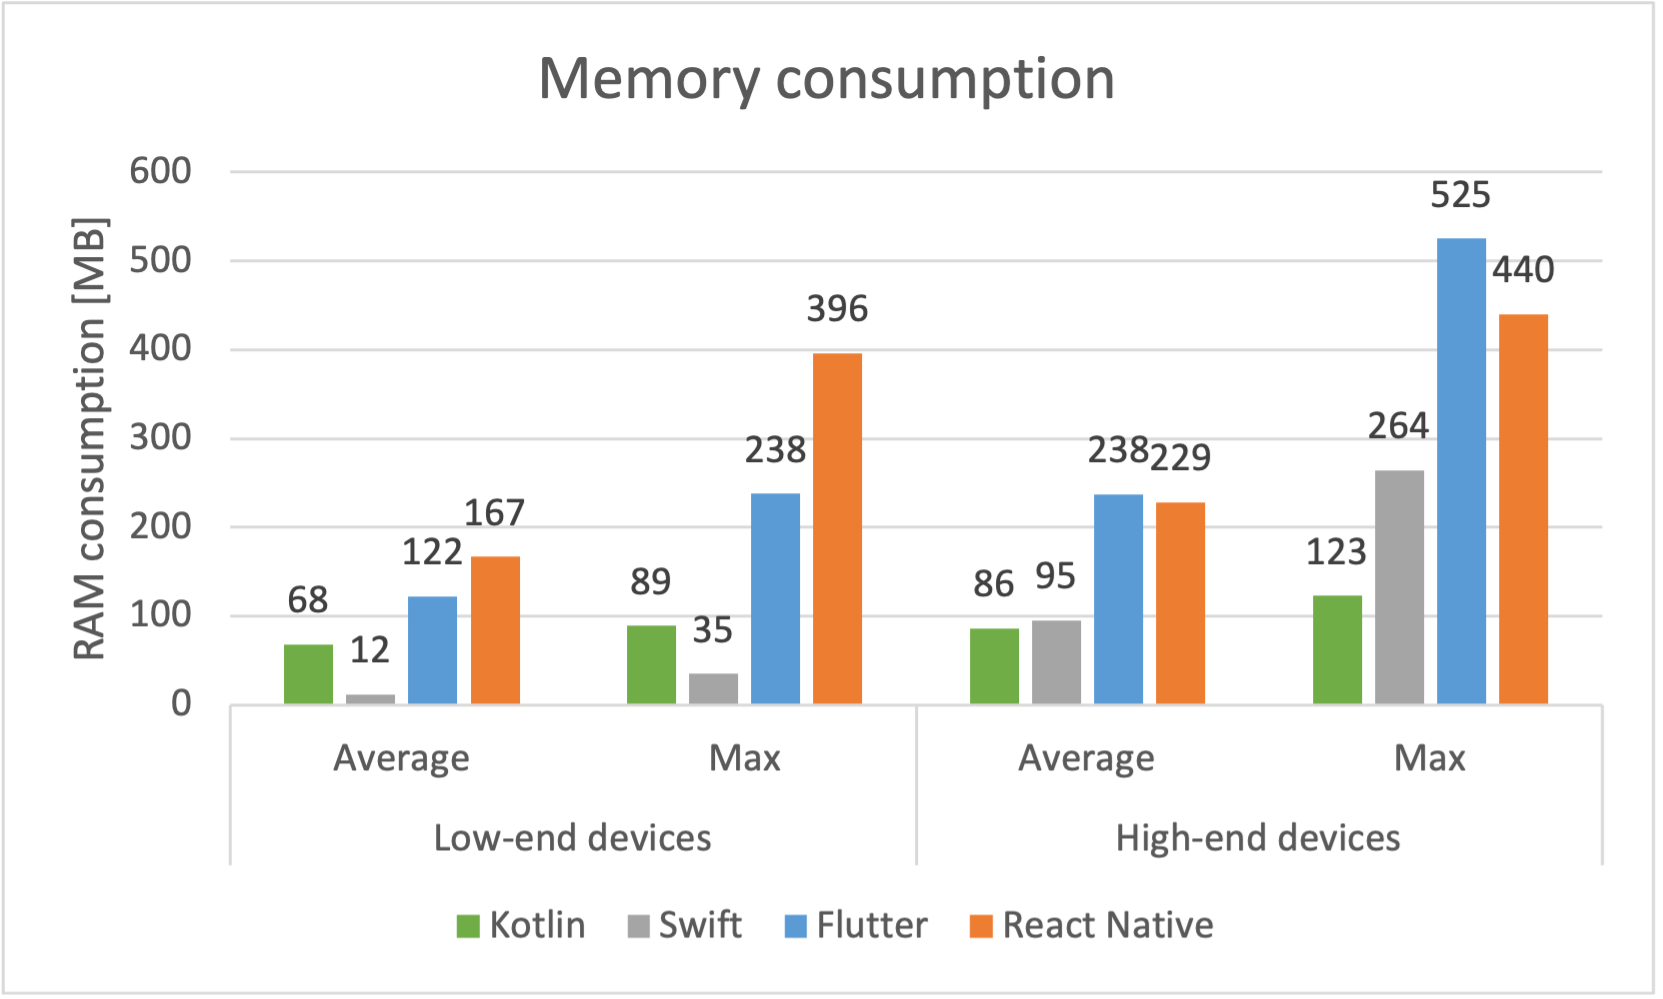
\includegraphics[width=.6\textwidth]{img/scenario3_ram}
    \caption{Research scenario 3: Memory consumption (Source: Own work)}
    \label{fig:s3_ram}
\end{figure}

Figure \ref{fig:s3_ram} shows the comparison of memory consumption among Android and iOS apps developed with Kotlin, Swift, Flutter, and React Native. On low-end devices, Swift apps heavily outperform other technologies; however, on high-end devices, Kotlin apps exhibit the lowest memory usage. Flutter and React Native apps demonstrate similar results. The former utilizes over 30\% less memory on low-end devices but about 4\% more on high-end devices. Analogously, Flutter apps experience smaller spikes on low-end devices and bigger spikes on high-end devices, reaching a maximum of over 500 MB.




\subsection{Research scenario 4 results analysis}

The following figures illustrate the aggregated results from the experiments conducted within Research scenario 4 described in Chapter \ref{chap:research_scenarios}.

\begin{figure}[H]
    \begin{minipage}{.48\textwidth}
        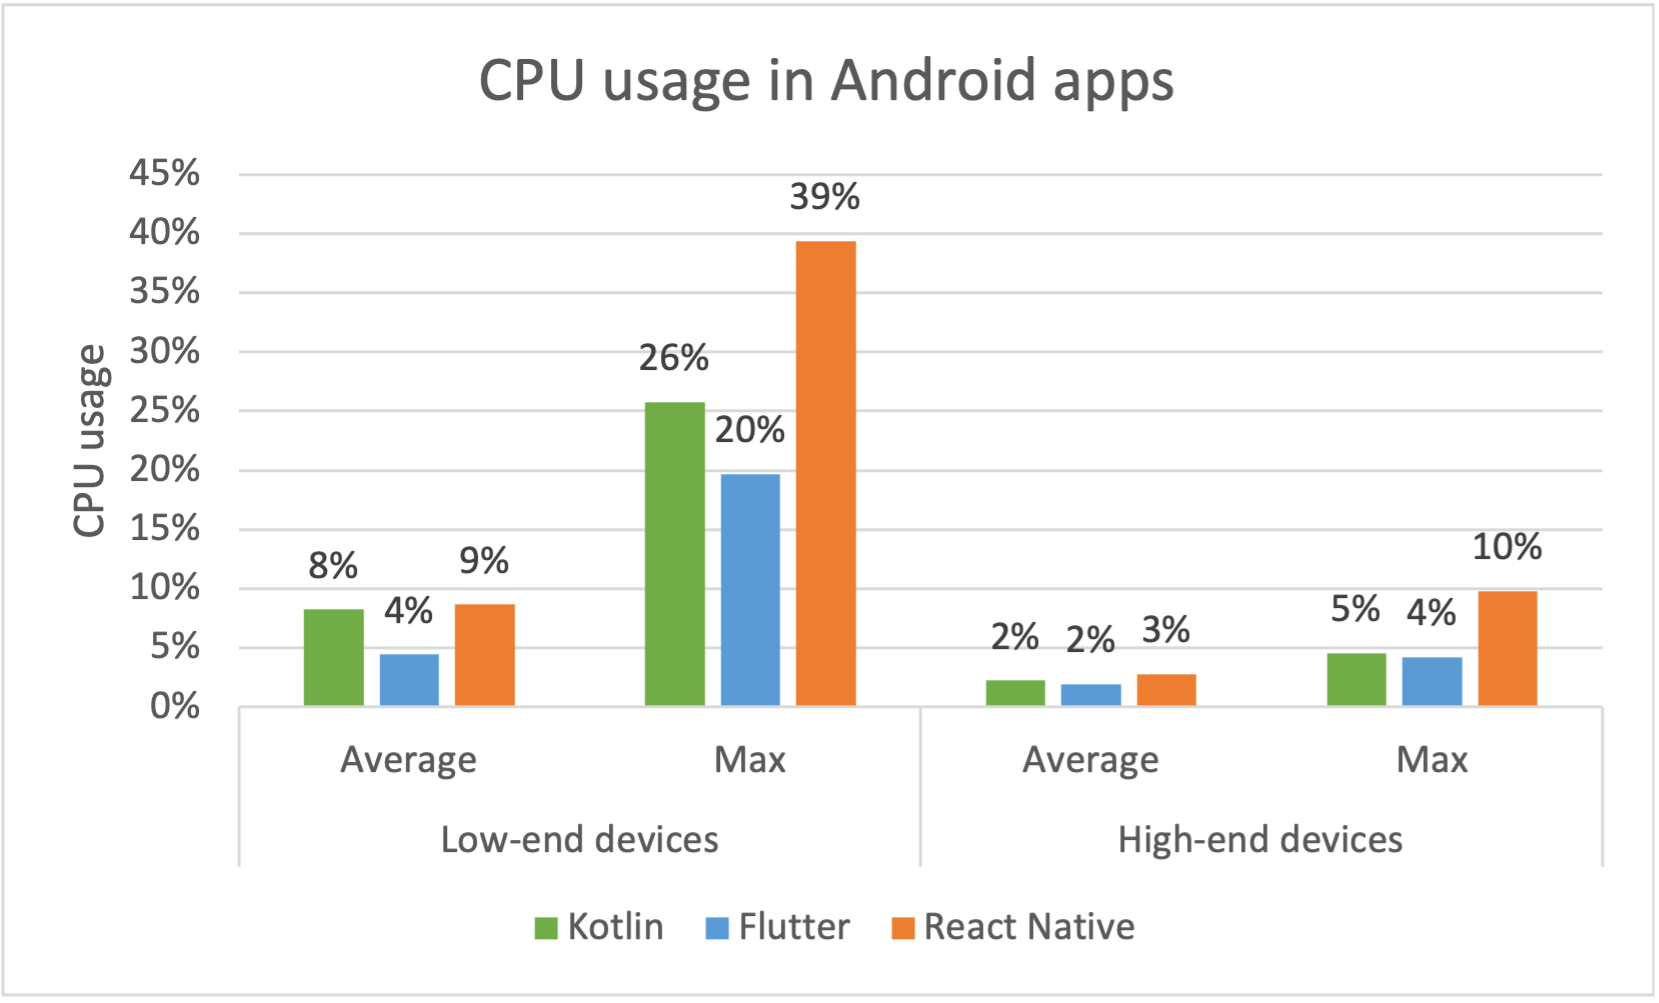
\includegraphics[width=\textwidth]{img/scenario4_cpu_android}
        \caption{Research scenario 4: CPU usage in Android apps (Source: Own work)}
        \label{fig:s4_cpu_android}
    \end{minipage}
    \hfill
    \begin{minipage}{.48\textwidth}
        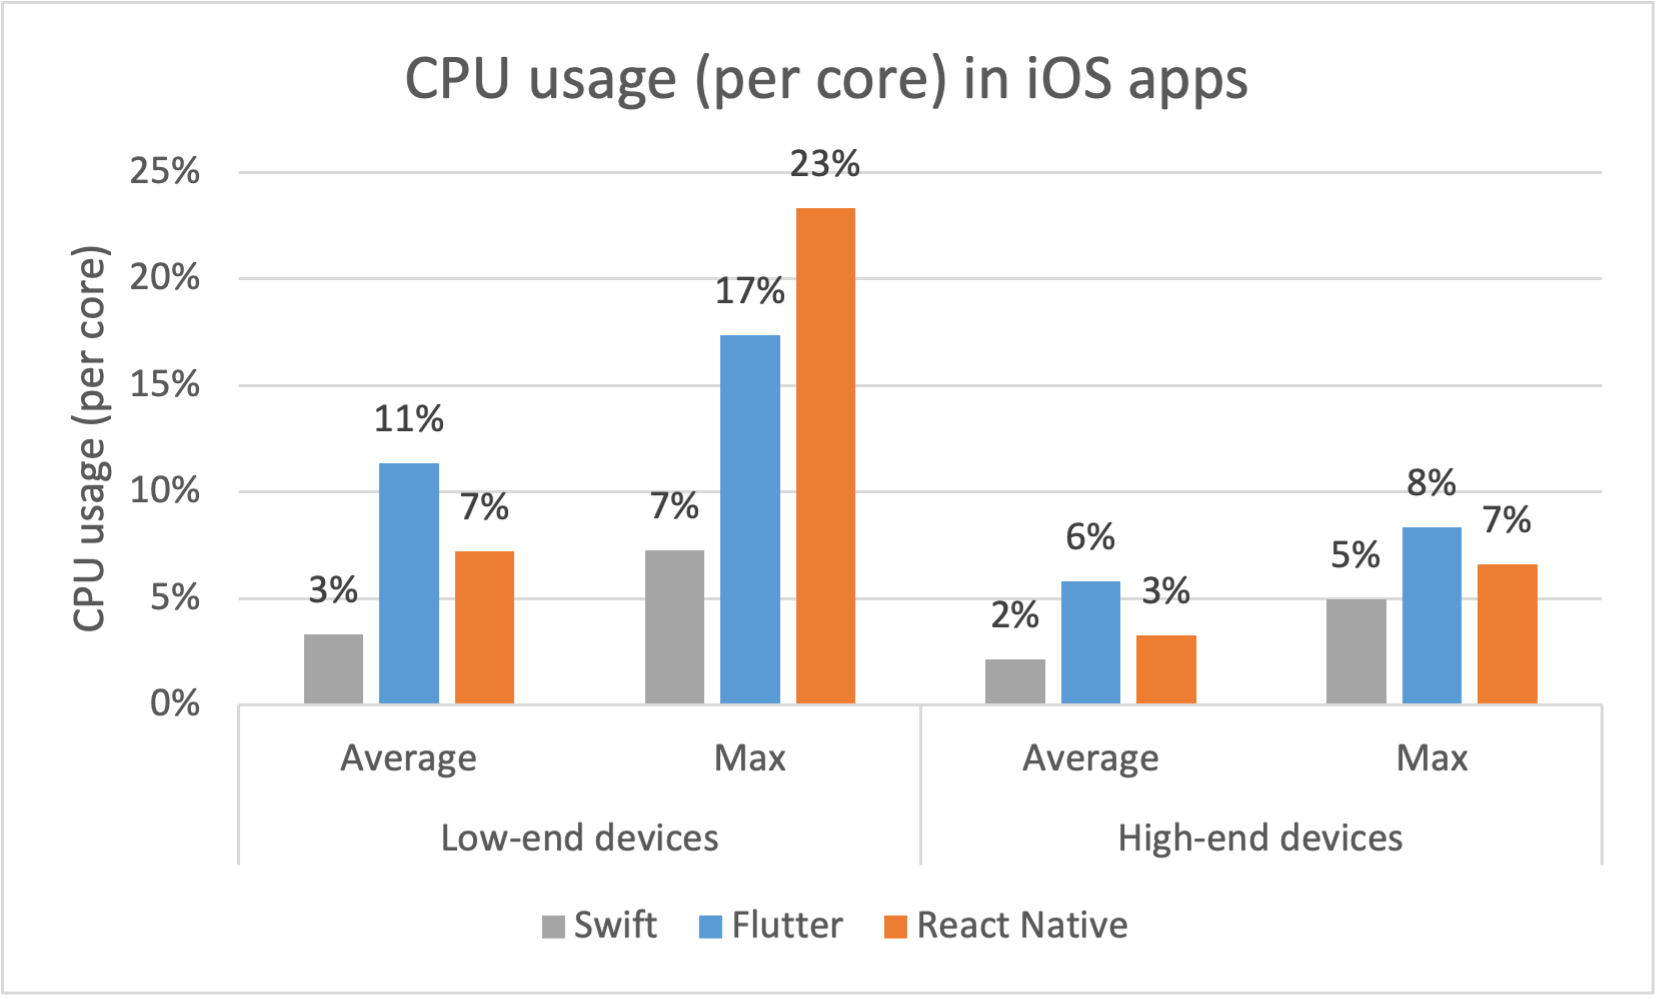
\includegraphics[width=\textwidth]{img/scenario4_cpu_ios}
        \caption{Research scenario 4: CPU usage in iOS apps (Source: Own work)}
        \label{fig:s4_cpu_ios}
    \end{minipage}
\end{figure}

Figures \ref{fig:s4_cpu_android} and \ref{fig:s4_cpu_ios} show the comparison of CPU usage among Android and iOS apps developed with Kotlin, Swift, Flutter, and React Native. On both platforms, the three technologies considered demonstrate similar CPU usage within the threshold of 2-10\% on high-end devices. On low-end Android devices, Flutter requires the least CPU capacity, while Kotlin and React Native achieve similar results, although React Native experiences higher spikes. Apps written in Swift exhibit the lowest CPU load on lower-end iOS devices. On average, React Native apps utilize less CPU resources than Flutter; however, they suffer from lower stability with spikes of 23\%.

\begin{figure}[H]
    \centering
    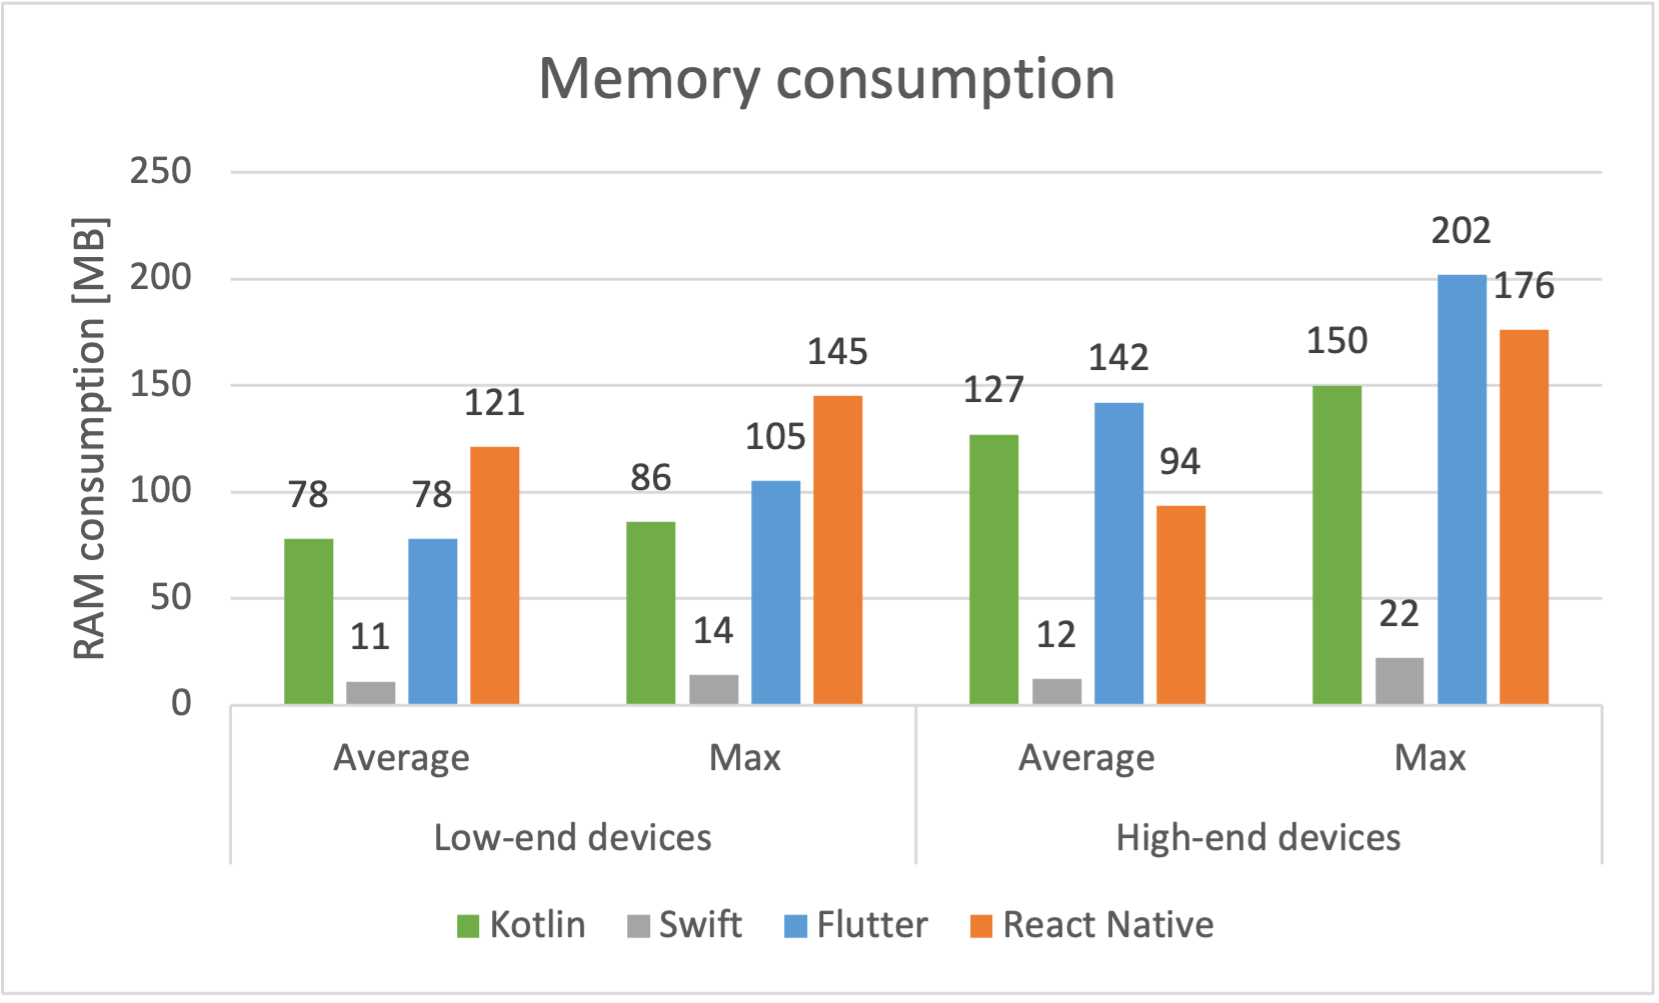
\includegraphics[width=.6\textwidth]{img/scenario4_ram}
    \caption{Research scenario 4: Memory consumption (Source: Own work)}
    \label{fig:s4_ram}
\end{figure}

Figure \ref{fig:s4_ram} shows the comparison of memory consumption among Android and iOS apps developed with Kotlin, Swift, Flutter, and React Native. It can be observed that Swift apps utilize significantly less memory than other technologies, maintaining consumption within the threshold of 11--22 MB. Kotlin and Flutter apps achieve similar performance on both low-end and high-end devices. On the other hand, React Native apps exhibit higher RAM usage on low-end devices but lower usage on high-end devices.


\section{Conclusions}

According to the literature review combined with the conducted experiments, cross- -platform development is a strong alternative to the native approach. The ability to utilize a single code base and deploy the application on more than one platform seems very efficient from the perspective of resource management, in both financial and timescale aspects. The concerns connected to cross-platform technologies come from their assumed inferiority to their native equivalents in the context of app performance and, thus, user experience, which is currently a top priority in mobile development. Nevertheless, the results from the experiments carried out in this thesis seem to at least partly invalidate those concerns. For example, even though native apps usually demonstrate lower memory usage on average, in many cases, cross-platform apps (especially those implemented with Flutter) achieve better results in the context of CPU usage and power consumption. When it comes to the frame rate, directly corresponding to the perceived smoothness, both native and cross-platform solutions performed similarly, except for Kotlin apps suffering from FPS drops on low-end devices.

Table \ref{best_framework} contains an overview of the best-performing development technologies grouped by research scenarios, performance metrics, target platforms, and device types. Each technology is represented by its abbreviation: Kotlin -- K, Swift -- S, Flutter -- F, and React Native -- RN. According to the information this table provides, the process of selecting a development method should become easier. One should consider the functionalities that must be implemented and compare them with the research scenarios considered in this thesis. Research scenario 1 related to one of the most common mobile application elements, which is the scrollable and filterable list. Research scenario 2 related to animations, which are responsible for a big part of user perception of a mobile application. Research scenario 3 related to file input and output, which is a very common feature found in many mobile applications. Research scenario 4 related to the functionality of user-controlled elements, e.g., switches and text fields, as well as the navigation between mobile application pages.

\clearpage

\begin{longtblr}[
    caption = {Best performing development solutions (Source: Own work)},
    label = {best_framework},
]{ colspec = { |c|c|c|c|c|c|c| }, hlines }
    \SetCell[c=3]{c}{\textbf{Variable}}&&&\textbf{Scenario 1}&\textbf{Scenario 2}& \textbf{Scenario 3}&\textbf{Scenario 4}\\
    
    \SetCell[r=4]{c}{CPU}&\SetCell[r=2]{c}{Android}&Low-end&F&K, F&K&F\\
    &&High-end&F, K&F, RN&K&K, F\\
    &\SetCell[r=2]{c}{iOS}&Low-end&S, F&S&S&S\\
    &&High-end&S, F&RN&S&S\\

    \SetCell[r=4]{c}{RAM}&\SetCell[r=2]{c}{Android}&Low-end&F&F&K&K, F\\
    &&High-end&K&F&K&RN\\
    &\SetCell[r=2]{c}{iOS}&Low-end&S&S&S&S\\
    &&High-end&S&S&S&S\\

    \SetCell[r=4]{c}{FPS}&\SetCell[r=2]{c}{Android}&Low-end&F&F, RN&--&--\\
    &&High-end&F&F, RN&--&--\\
    &\SetCell[r=2]{c}{iOS}&Low-end&F&S&--&--\\
    &&High-end&F&S, F, RN&--&--\\
\end{longtblr}

The research carried out for the purpose of this master's thesis leads to the following conclusions:

\begin{itemize}
    \item On average, Flutter provides the best performance out of all the technologies considered.
    \item Kotlin and Flutter apps require similar CPU usage, mutually outperforming each other in different scenarios.
    \item In most cases, Kotlin utilizes the least device memory in Android apps.
    \item Flutter seems to offer the best frame rate results with a high degree of stability, which may be caused by the usage of a new rendering engine \emph{Impeller}.
    \item Flutter applications exhibit the highest memory consumption, which may be an issue when considering low-end devices.
    \item In the considered scenarios, React Native offers the lowest overall performance.
    \item Swift offers great performance in every aspect; therefore, if a mobile application does not have to be multi-platform, it is a great choice, especially considering the excellent memory consumption levels.
\end{itemize}

\clearpage
